\documentclass[11pt,a4paper]{article}

\usepackage{graphicx}
\usepackage{lmodern}
\usepackage[T1]{fontenc}
\usepackage[utf8]{inputenc}
\usepackage{booktabs}
\usepackage{listings}
\usepackage{hyperref}
\usepackage{geometry}
\geometry{margin=1in}
\usepackage{caption}

\setlength\parindent{0pt}
\setlength{\parskip}{1em}

\title{\textbf{PG-MambaGAN Training Diagnostic Report} \\ \Large Epoch 10 Status Analysis \\ \vspace{0.5em} \textbf{PG-MambaGAN Eğitim Teşhis Raporu} \\ \Large 10. Epoch Durum Analizi}
\author{Autonomous Analysis System / Otonom Analiz Sistemi}
\date{\today}

\begin{document}

\maketitle

\vspace{1em}
\noindent\fbox{\parbox{\dimexpr\textwidth-2\fboxsep-2\fboxrule\relax}{
\textbf{Analysis Objective / Analiz Amacı:} \\
\textbf{EN:} This report provides a mid-training diagnostic snapshot (at Epoch 10) of the \textbf{PG-MambaGAN} model. The primary goal is to empower an analysis agent (or human reviewer) to determine whether to continue training under the current configuration, halt early, or modify the architecture/hyperparameters. Please review the quantitative metrics (loss curves, learning rates) and qualitative outputs (generated images) to formulate a final verdict. \\
\textbf{TR:} Bu rapor, \textbf{PG-MambaGAN} modelinin eğitim ortası (10. Epoch) teşhis özetini sunmaktadır. Temel amaç, analiz ajanının (veya insan inceleyicinin) mevcut yapılandırmayla eğitime devam edip etmeme, erken durdurma veya mimari/hiperparametreleri değiştirme kararı vermesini sağlamaktır. Nihai kararı vermek için lütfen nicel metrikleri (kayıp eğrileri, öğrenme oranları) ve nitel çıktıları (üretilen görüntüler) inceleyin.
}}
\vspace{1em}

\clearpage
\section{Quantitative Training Metrics (W\&B Charts) / Nicel Eğitim Metrikleri}

\begin{figure}[!htb]
\centering
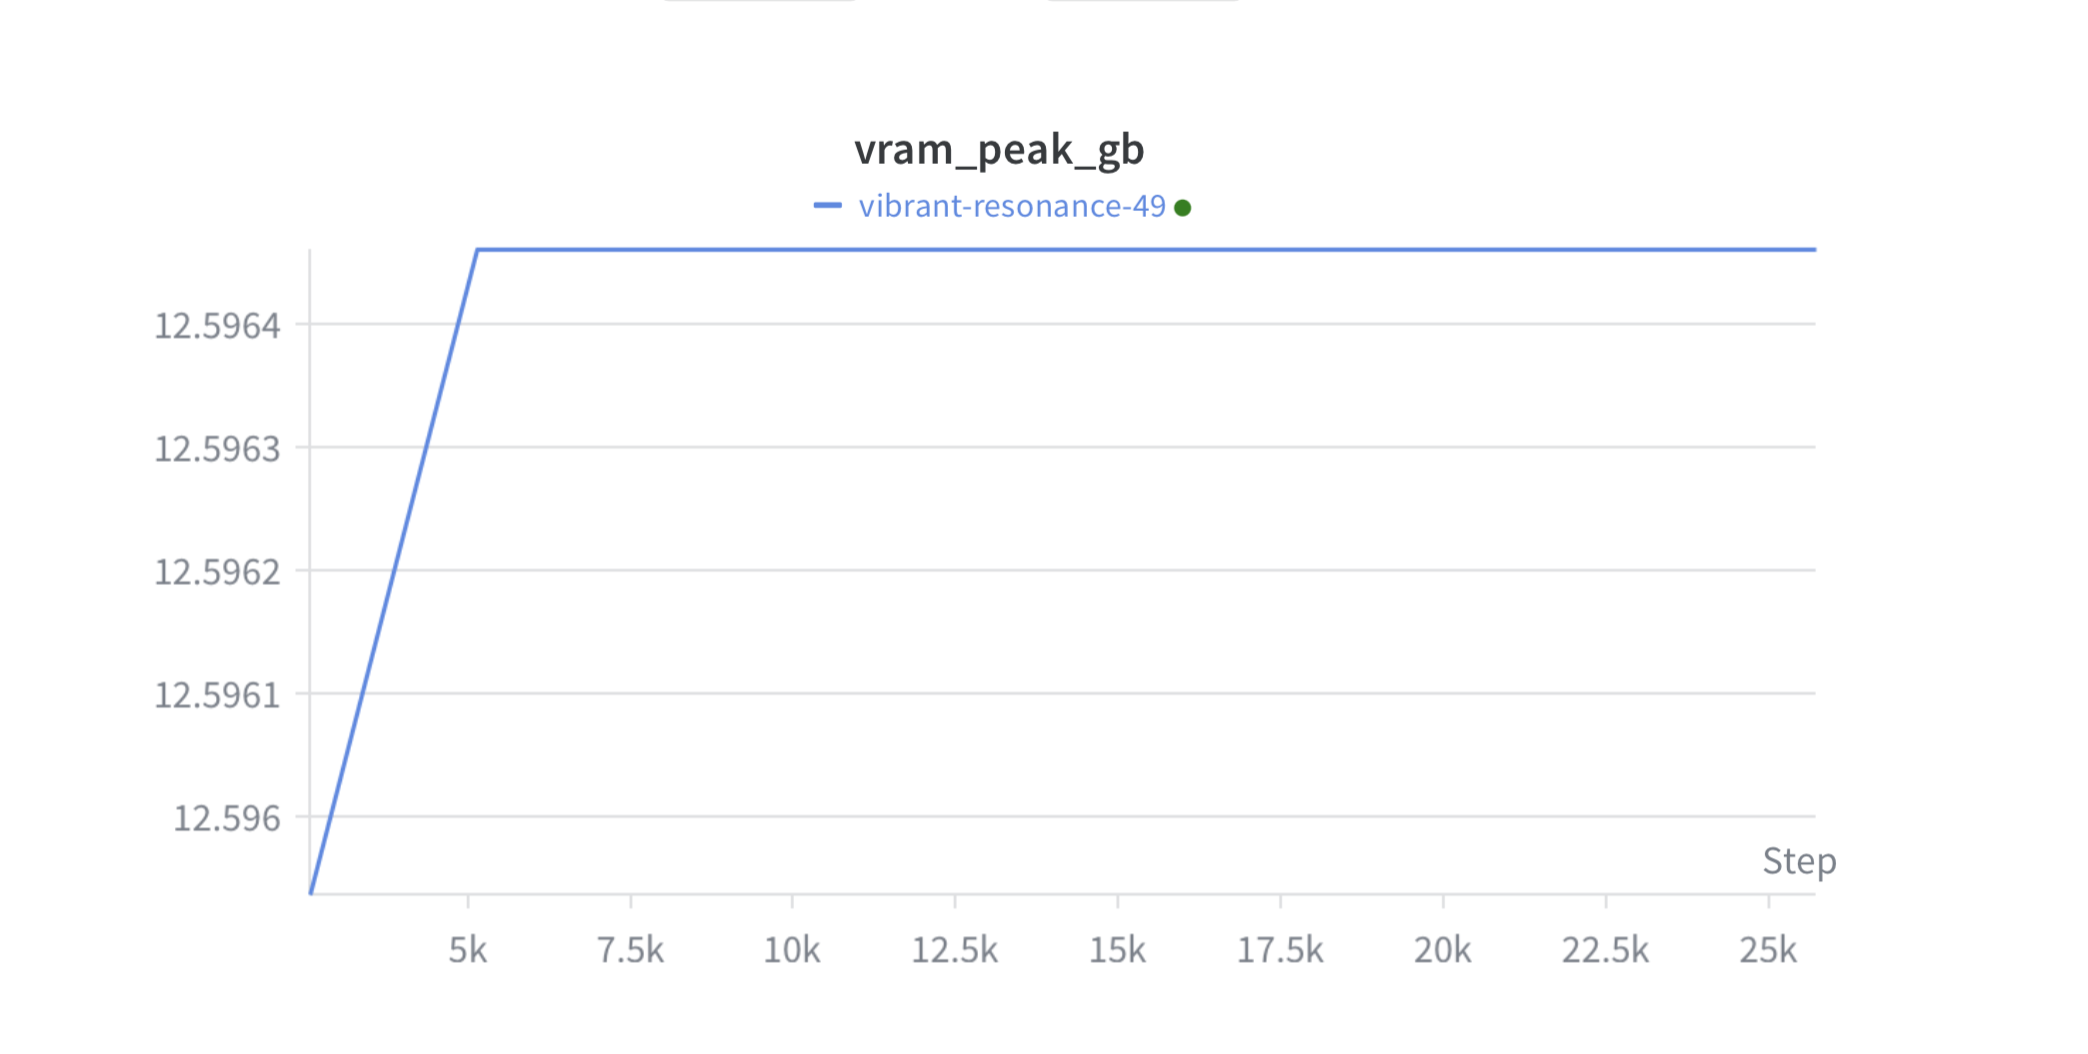
\includegraphics[width=0.95\textwidth]{charts/chart_01.png}
\caption{Metric Chart 1 / Metrik Grafiği 1}
\end{figure}
\begin{figure}[!htb]
\centering
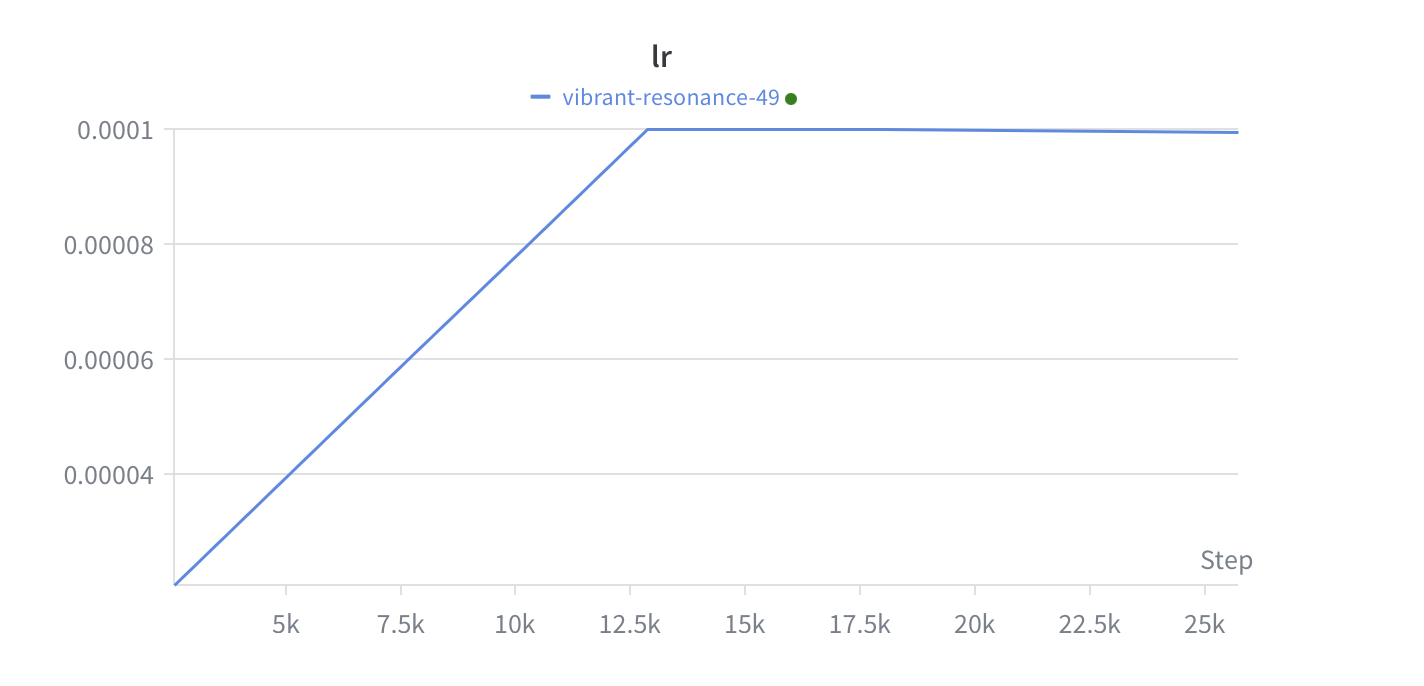
\includegraphics[width=0.95\textwidth]{charts/chart_02.png}
\caption{Metric Chart 2 / Metrik Grafiği 2}
\end{figure}
\clearpage
\begin{figure}[!htb]
\centering
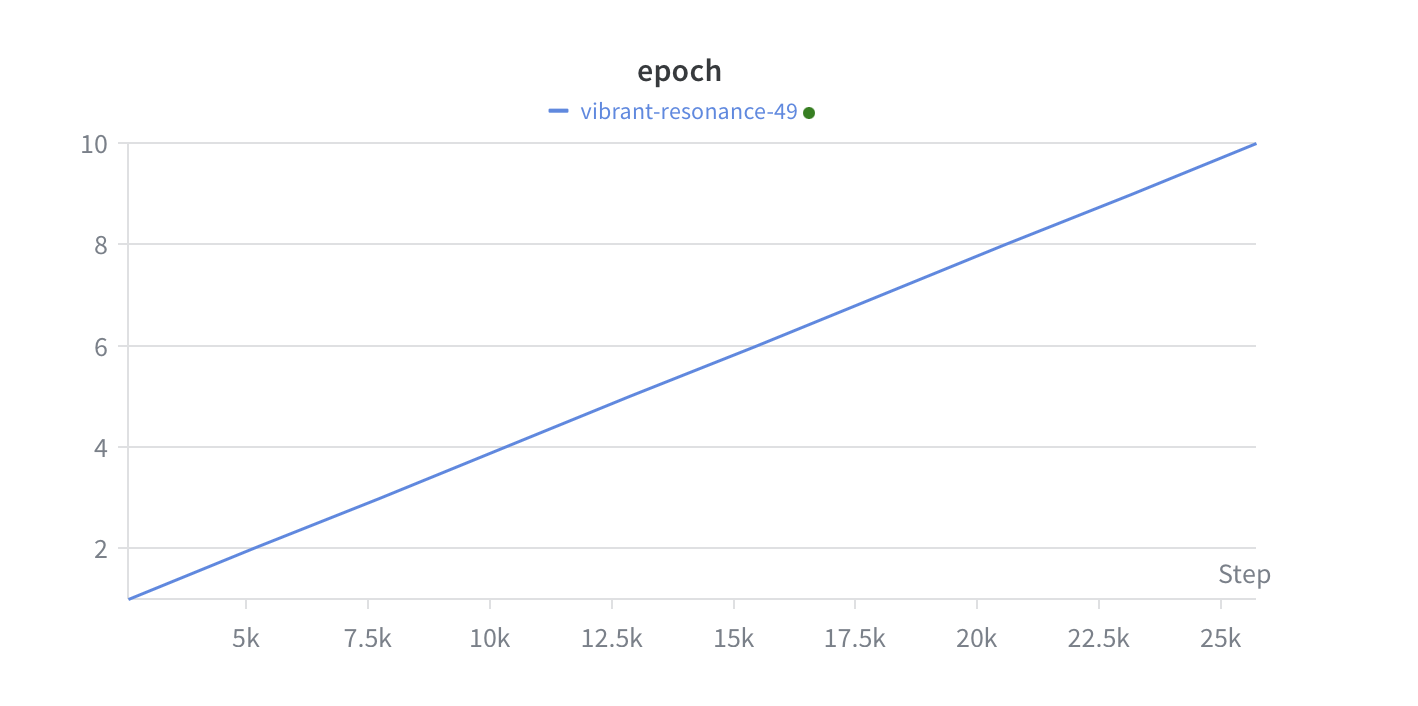
\includegraphics[width=0.95\textwidth]{charts/chart_03.png}
\caption{Metric Chart 3 / Metrik Grafiği 3}
\end{figure}
\begin{figure}[!htb]
\centering
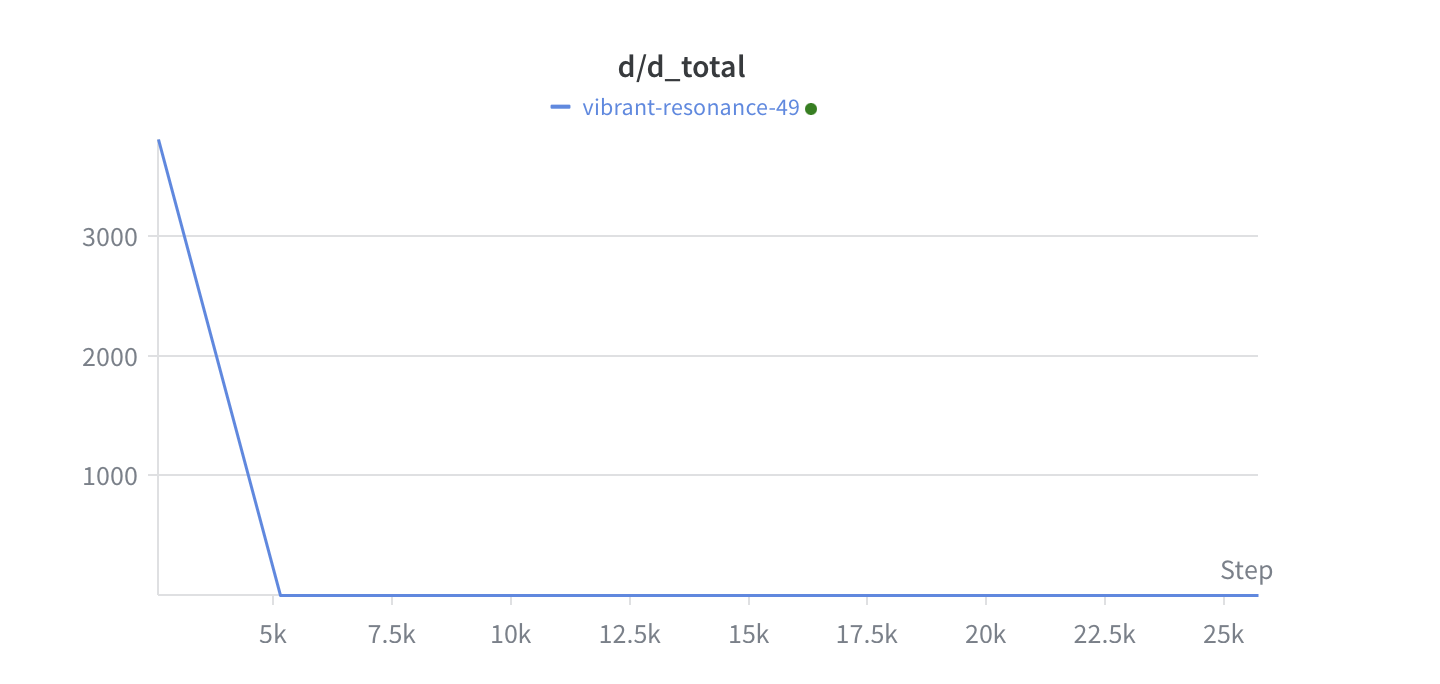
\includegraphics[width=0.95\textwidth]{charts/chart_04.png}
\caption{Metric Chart 4 / Metrik Grafiği 4}
\end{figure}
\clearpage
\begin{figure}[!htb]
\centering
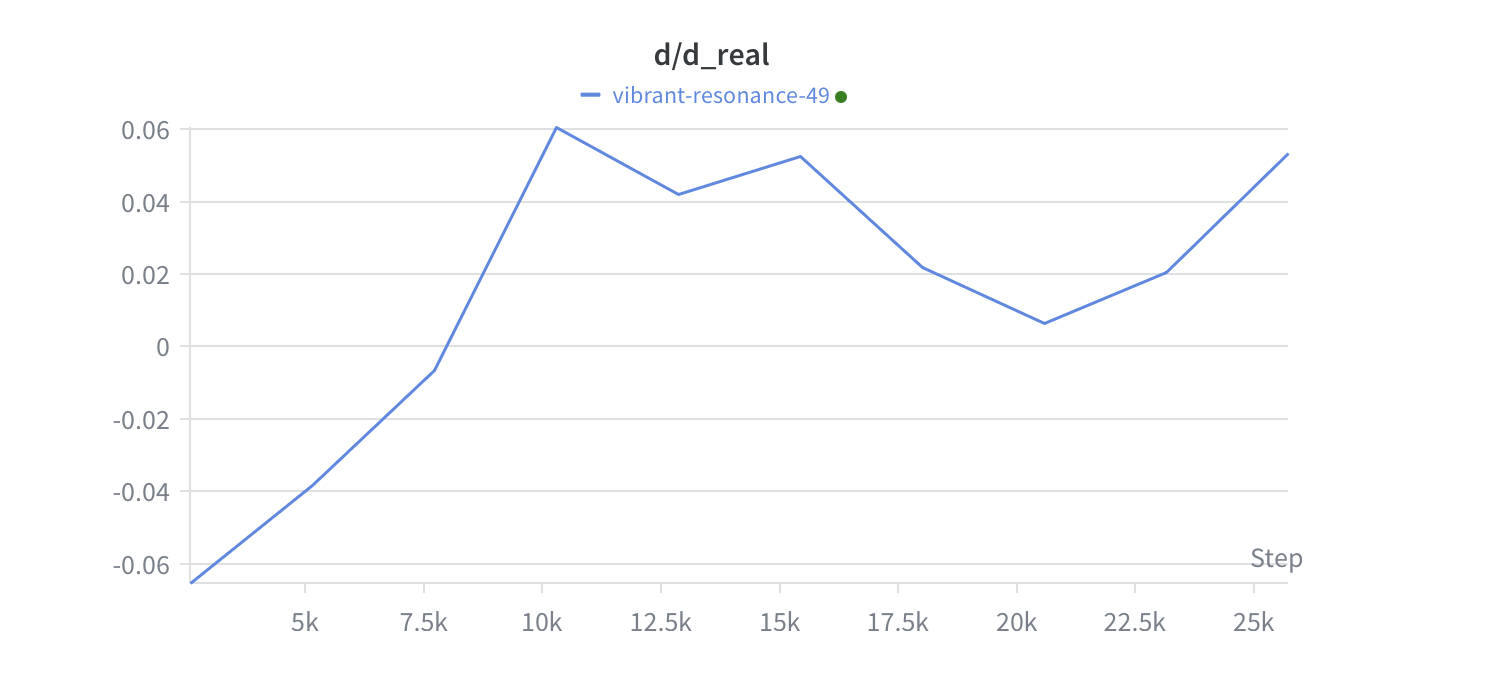
\includegraphics[width=0.95\textwidth]{charts/chart_05.png}
\caption{Metric Chart 5 / Metrik Grafiği 5}
\end{figure}
\begin{figure}[!htb]
\centering
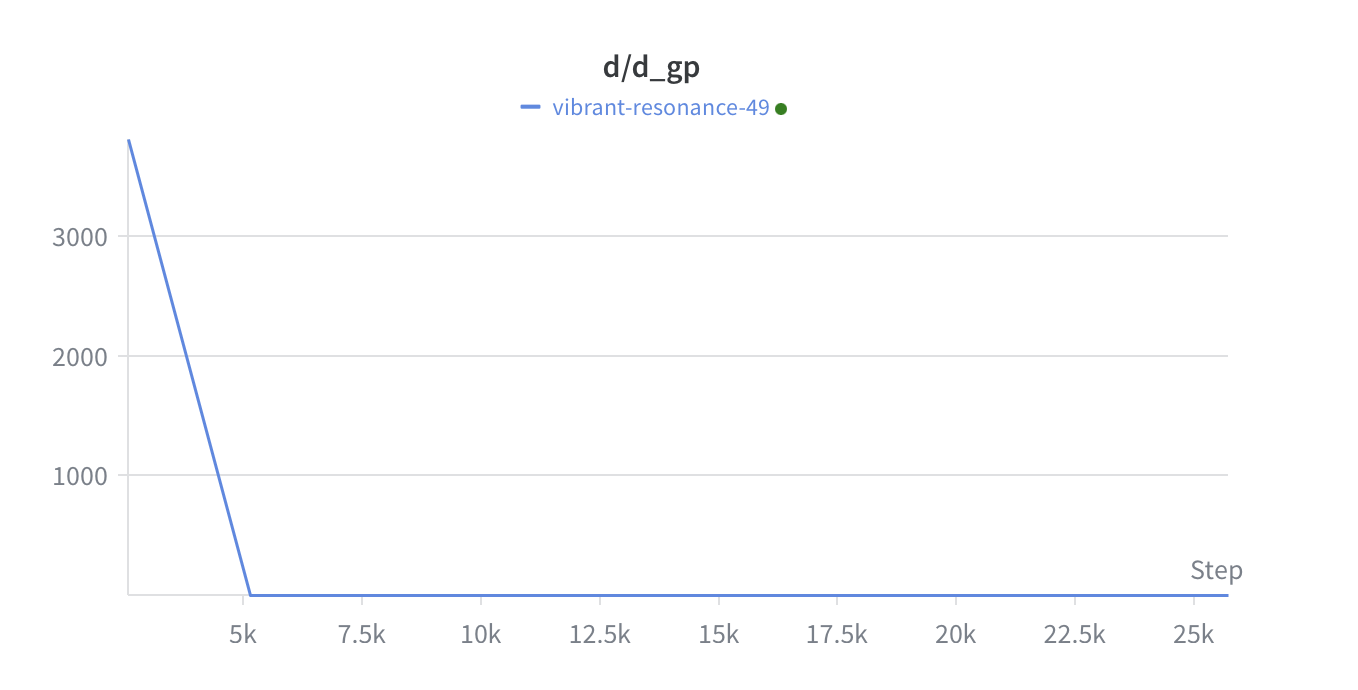
\includegraphics[width=0.95\textwidth]{charts/chart_06.png}
\caption{Metric Chart 6 / Metrik Grafiği 6}
\end{figure}
\clearpage
\begin{figure}[!htb]
\centering
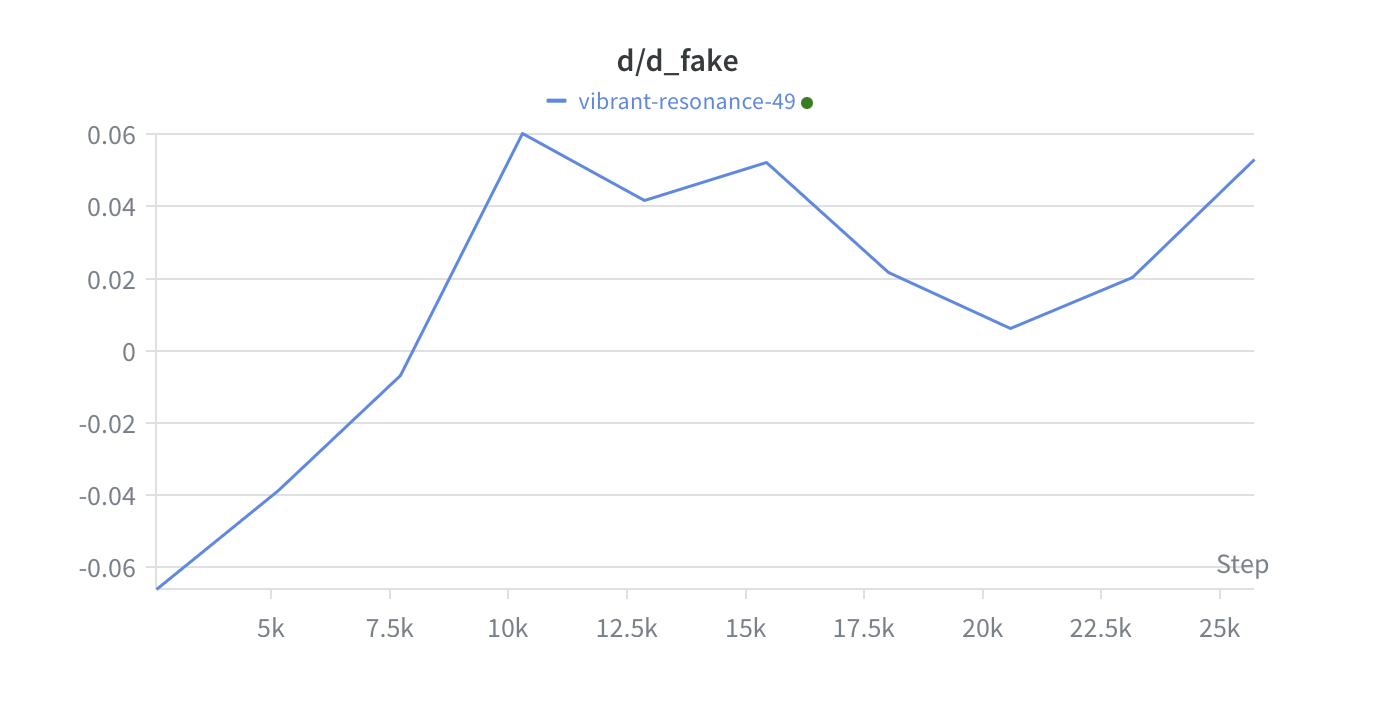
\includegraphics[width=0.95\textwidth]{charts/chart_07.png}
\caption{Metric Chart 7 / Metrik Grafiği 7}
\end{figure}
\begin{figure}[!htb]
\centering
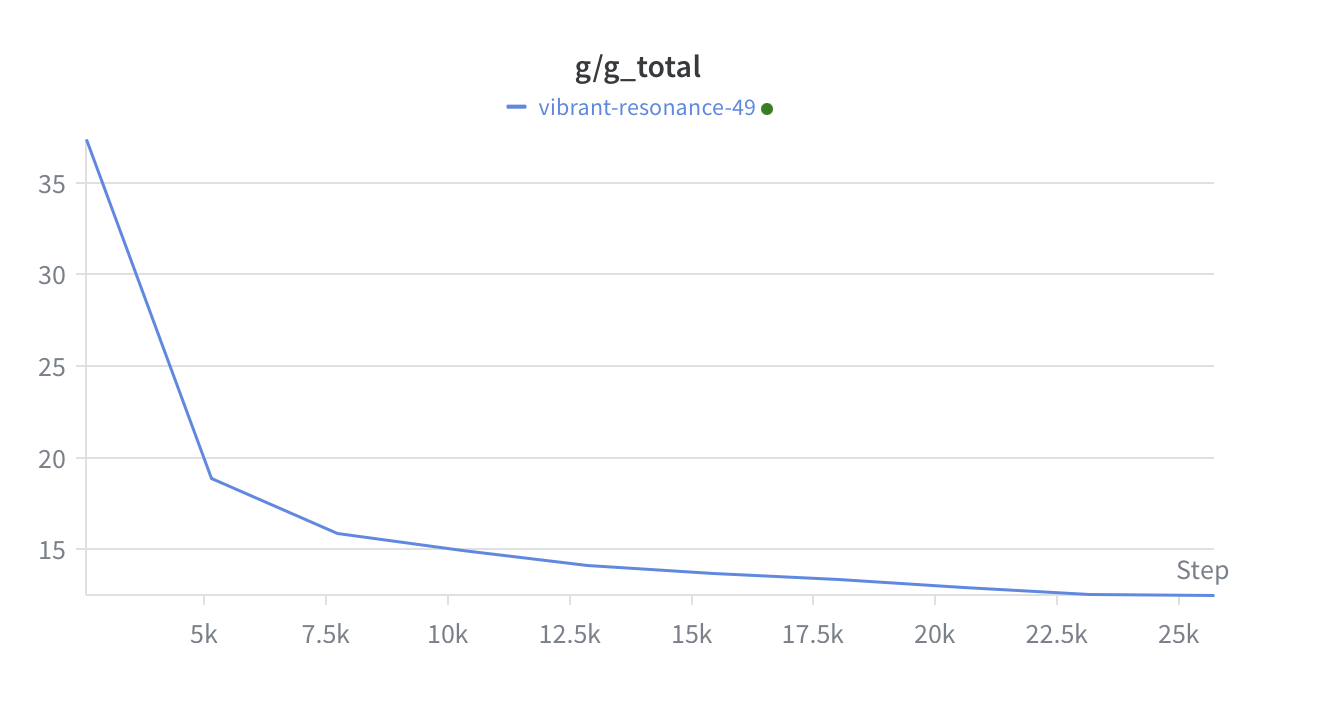
\includegraphics[width=0.95\textwidth]{charts/chart_08.png}
\caption{Metric Chart 8 / Metrik Grafiği 8}
\end{figure}
\clearpage
\begin{figure}[!htb]
\centering
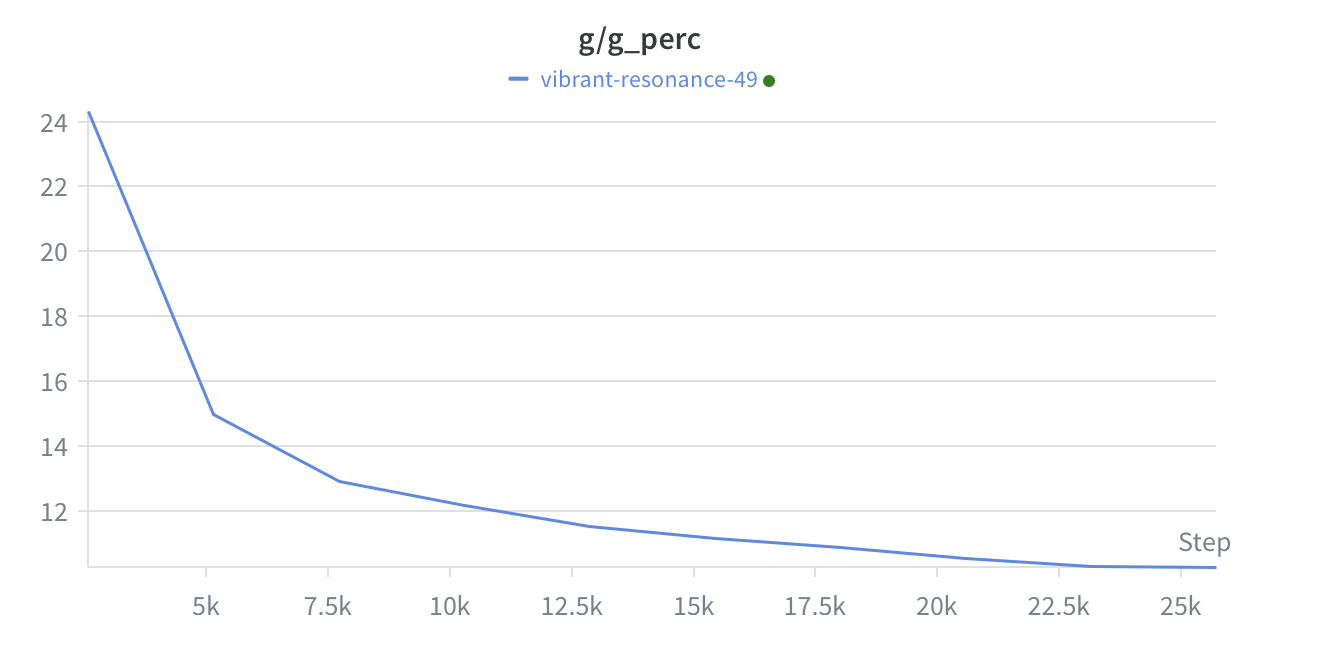
\includegraphics[width=0.95\textwidth]{charts/chart_09.png}
\caption{Metric Chart 9 / Metrik Grafiği 9}
\end{figure}
\begin{figure}[!htb]
\centering
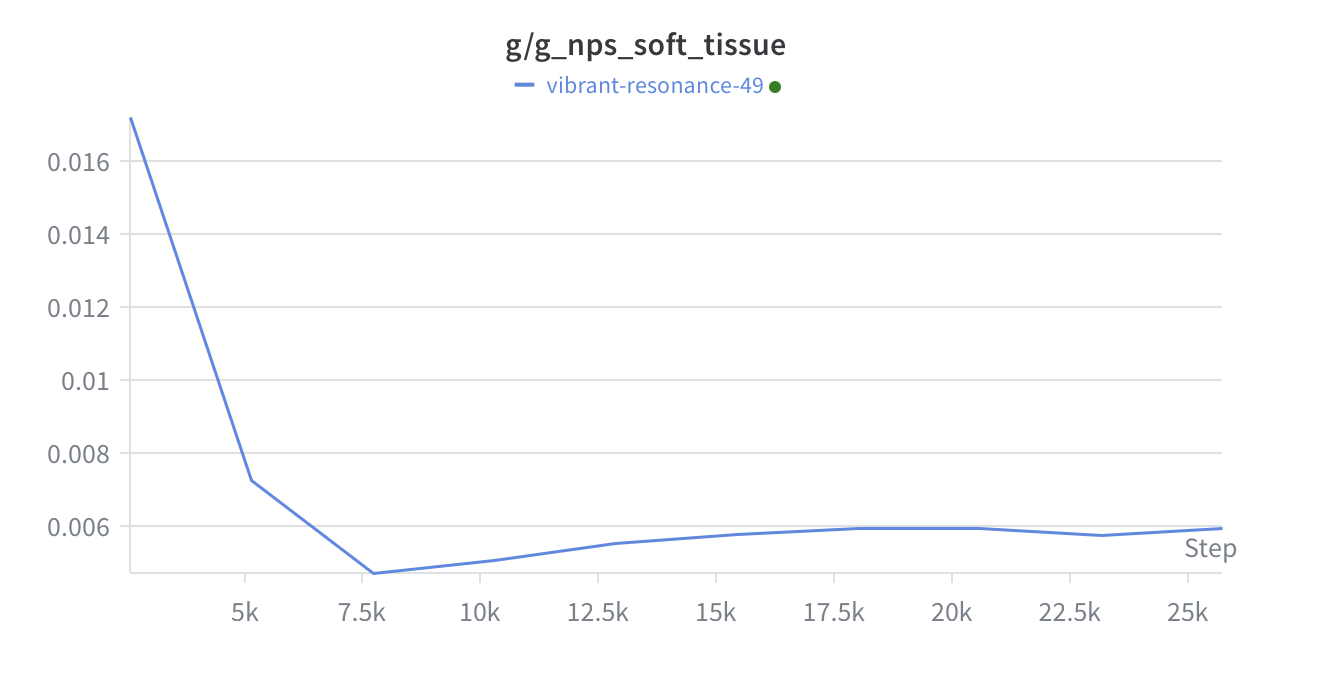
\includegraphics[width=0.95\textwidth]{charts/chart_10.png}
\caption{Metric Chart 10 / Metrik Grafiği 10}
\end{figure}
\clearpage
\begin{figure}[!htb]
\centering
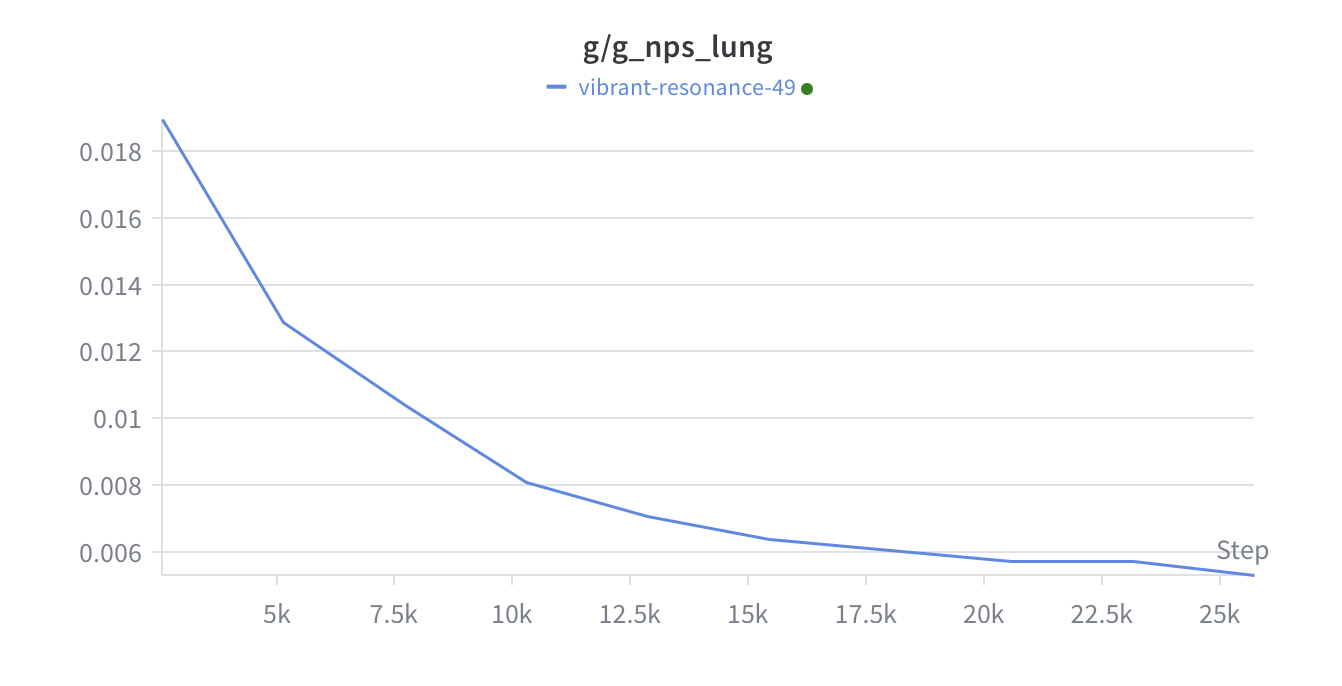
\includegraphics[width=0.95\textwidth]{charts/chart_11.png}
\caption{Metric Chart 11 / Metrik Grafiği 11}
\end{figure}
\begin{figure}[!htb]
\centering
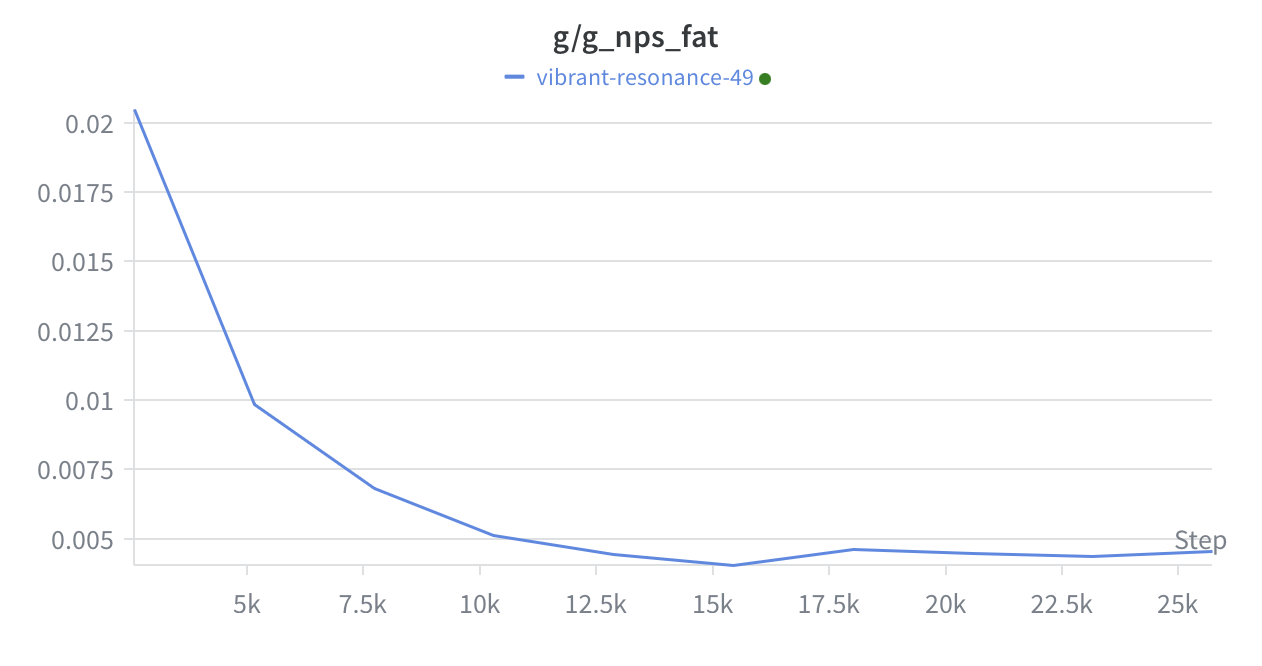
\includegraphics[width=0.95\textwidth]{charts/chart_12.png}
\caption{Metric Chart 12 / Metrik Grafiği 12}
\end{figure}
\clearpage
\begin{figure}[!htb]
\centering
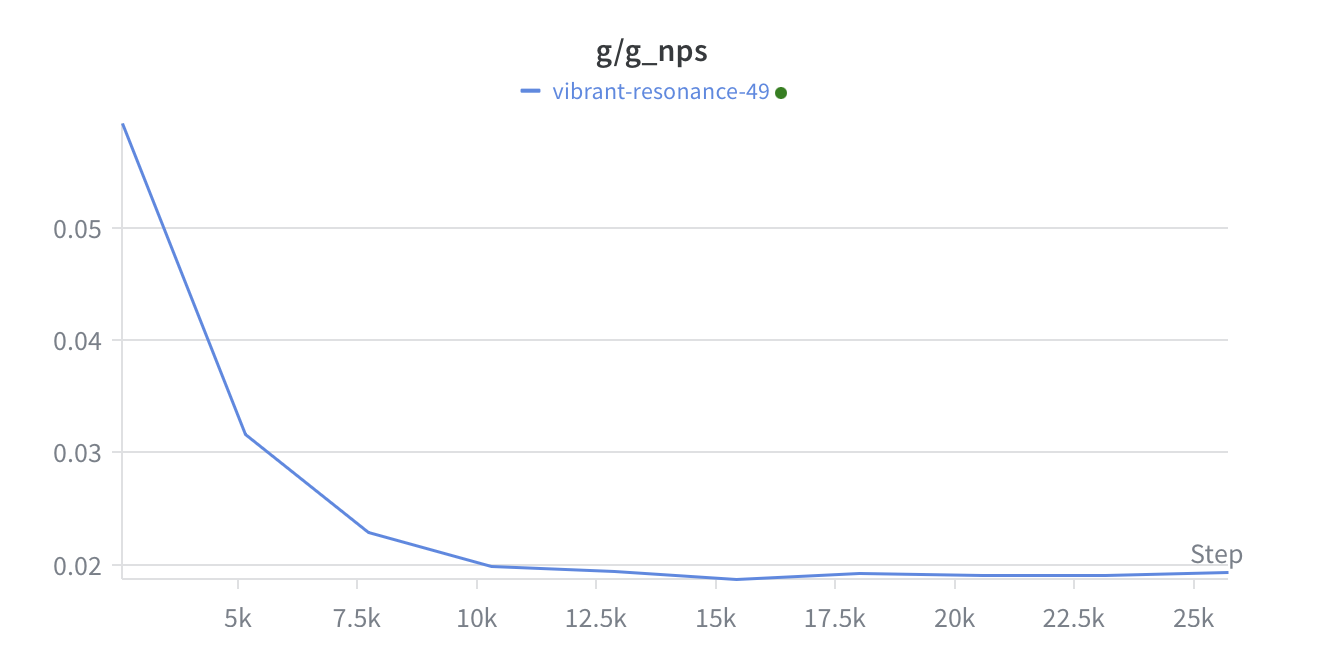
\includegraphics[width=0.95\textwidth]{charts/chart_13.png}
\caption{Metric Chart 13 / Metrik Grafiği 13}
\end{figure}
\begin{figure}[!htb]
\centering
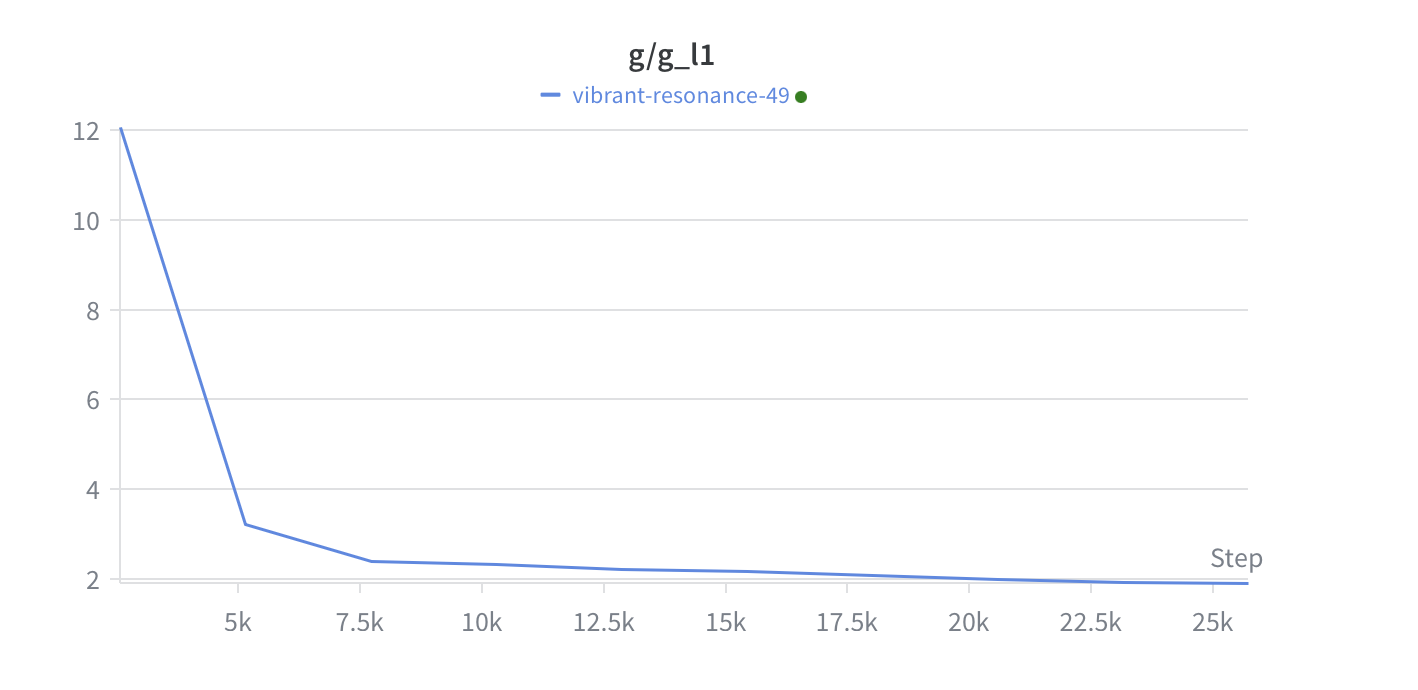
\includegraphics[width=0.95\textwidth]{charts/chart_14.png}
\caption{Metric Chart 14 / Metrik Grafiği 14}
\end{figure}
\clearpage
\begin{figure}[!htb]
\centering
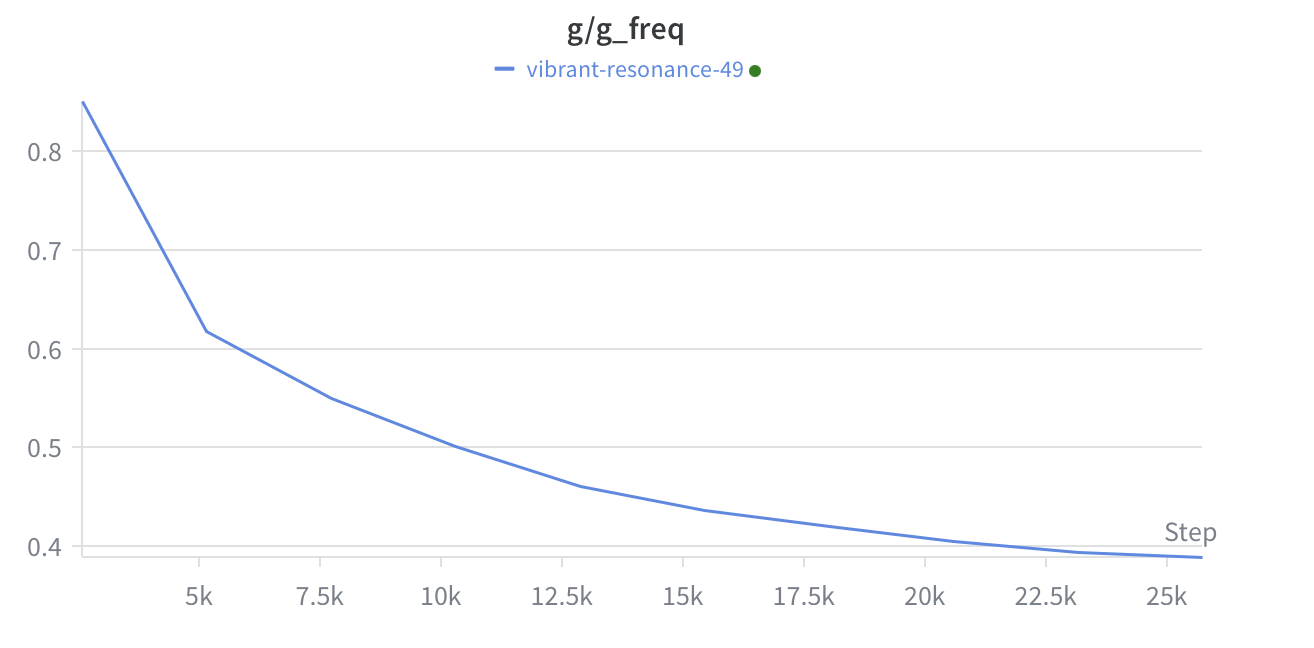
\includegraphics[width=0.95\textwidth]{charts/chart_15.png}
\caption{Metric Chart 15 / Metrik Grafiği 15}
\end{figure}
\begin{figure}[!htb]
\centering
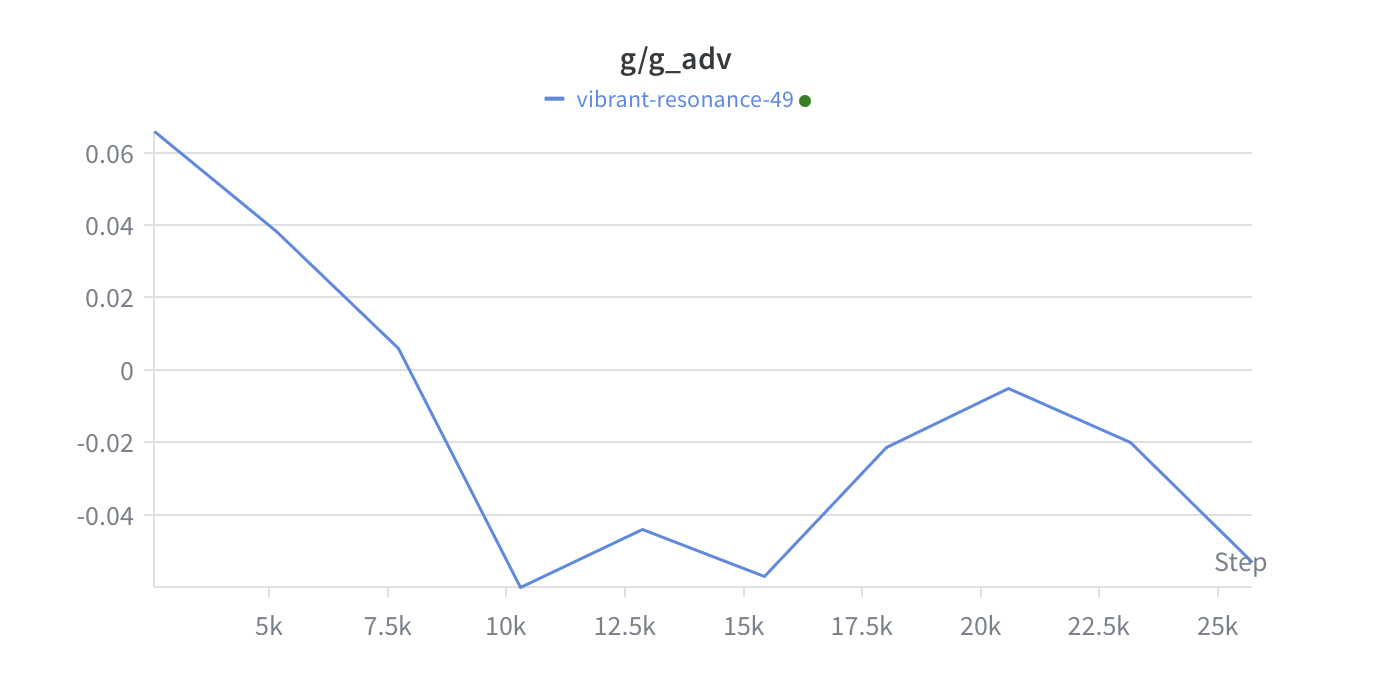
\includegraphics[width=0.95\textwidth]{charts/chart_16.png}
\caption{Metric Chart 16 / Metrik Grafiği 16}
\end{figure}
\clearpage
\begin{figure}[!htb]
\centering
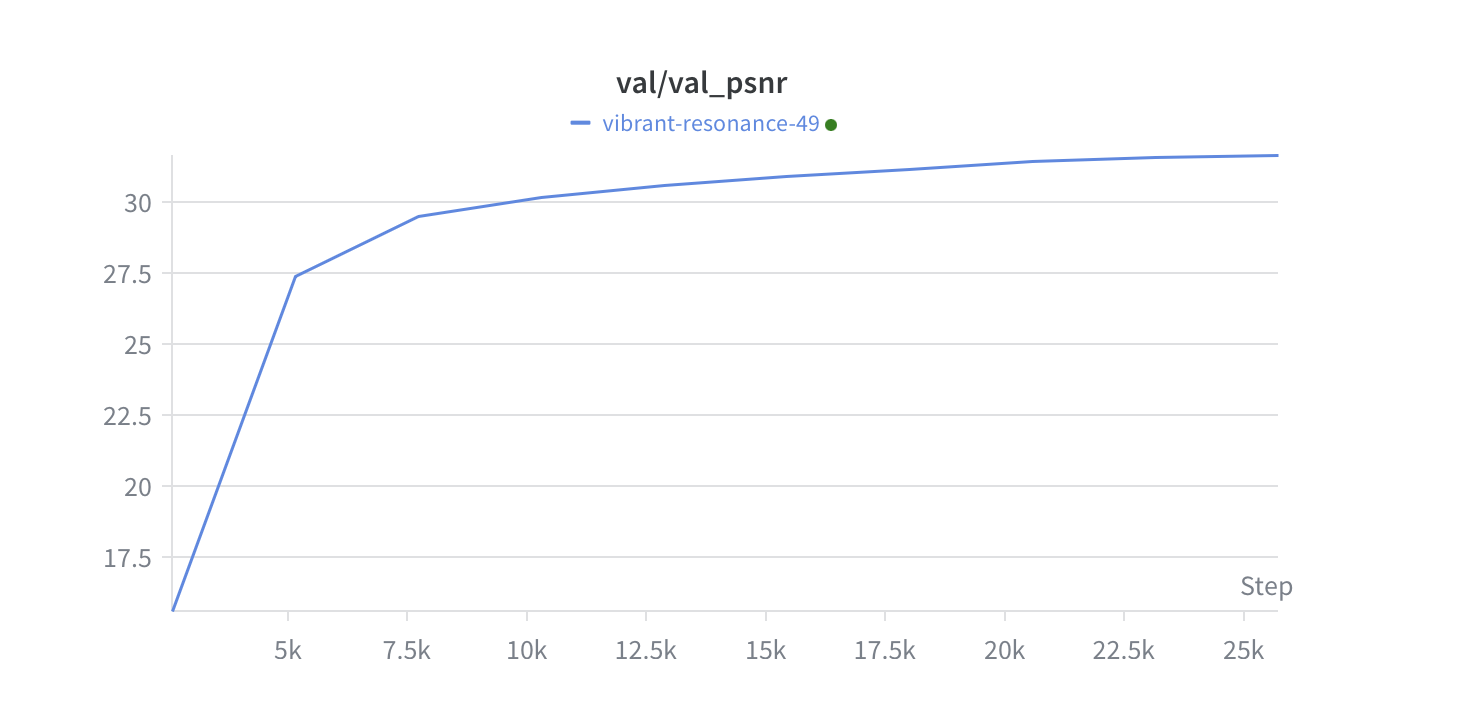
\includegraphics[width=0.95\textwidth]{charts/chart_17.png}
\caption{Metric Chart 17 / Metrik Grafiği 17}
\end{figure}
\begin{figure}[!htb]
\centering
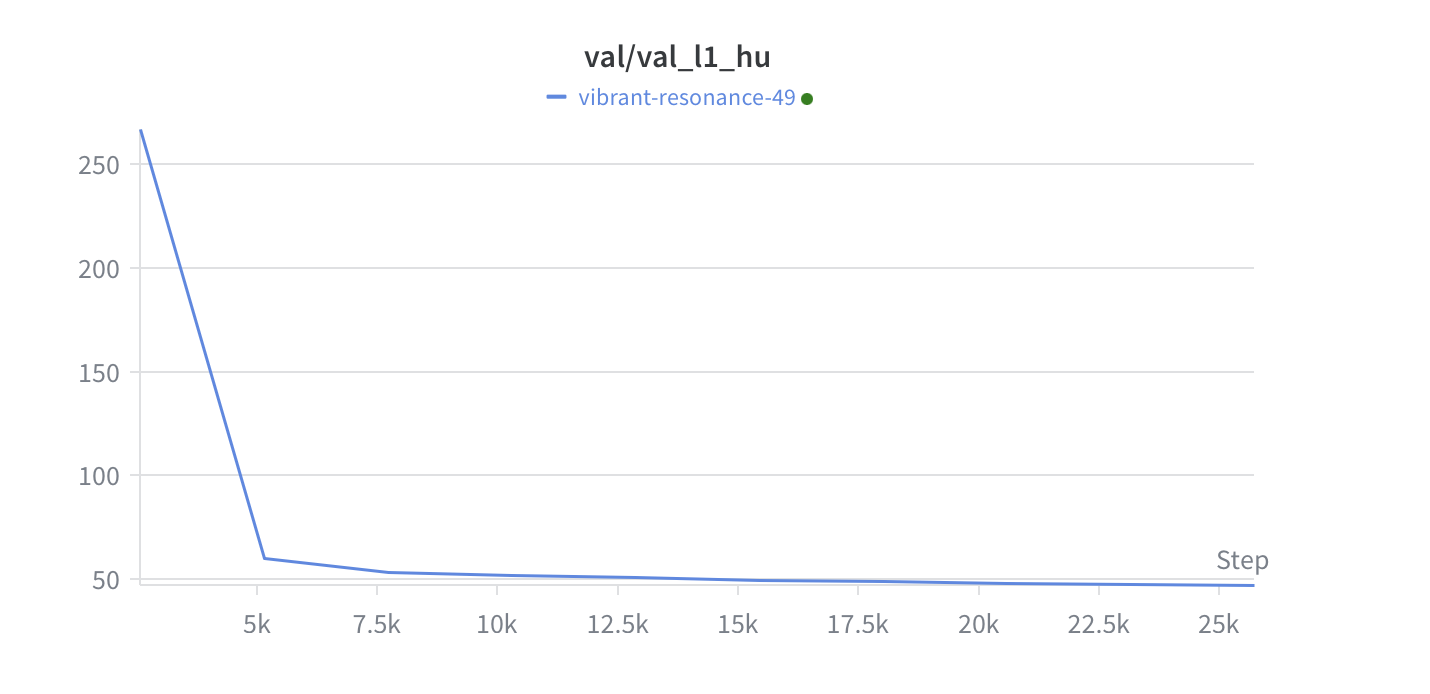
\includegraphics[width=0.95\textwidth]{charts/chart_18.png}
\caption{Metric Chart 18 / Metrik Grafiği 18}
\end{figure}
\clearpage
\begin{figure}[!htb]
\centering
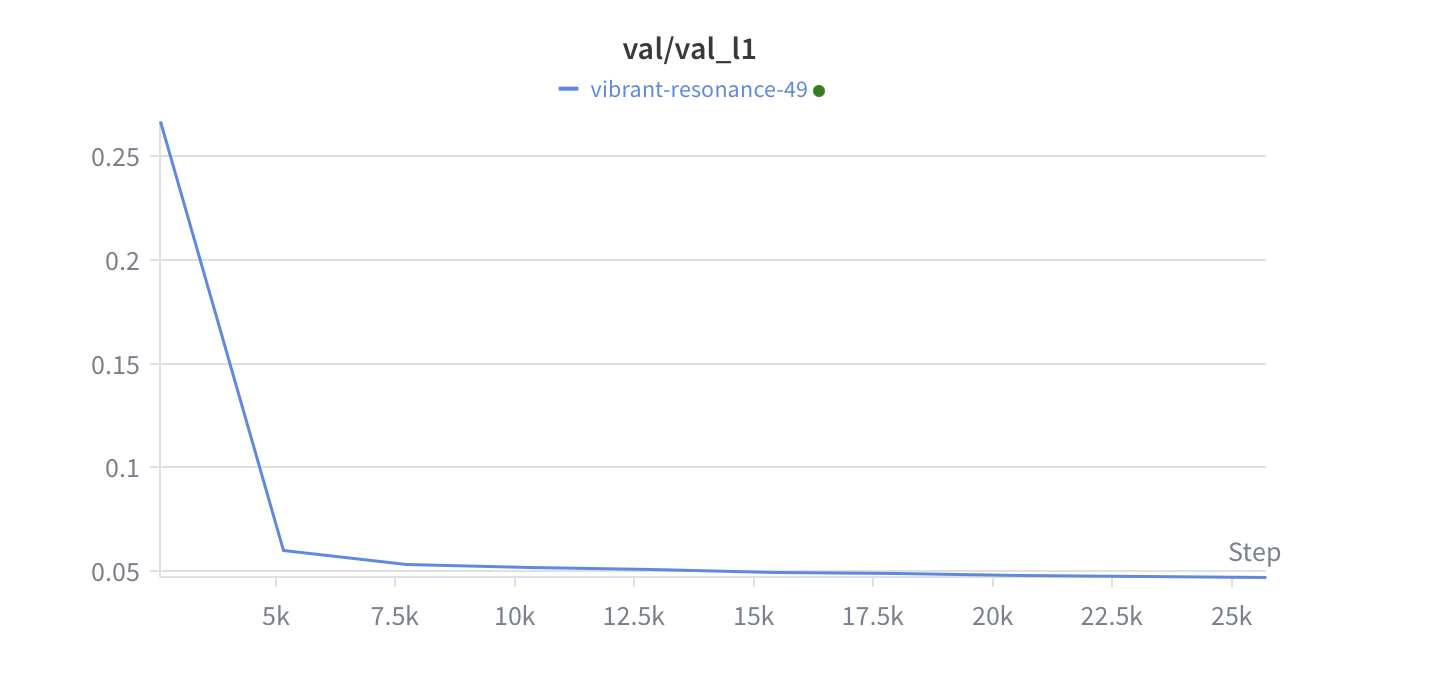
\includegraphics[width=0.95\textwidth]{charts/chart_19.png}
\caption{Metric Chart 19 / Metrik Grafiği 19}
\end{figure}
\begin{figure}[!htb]
\centering
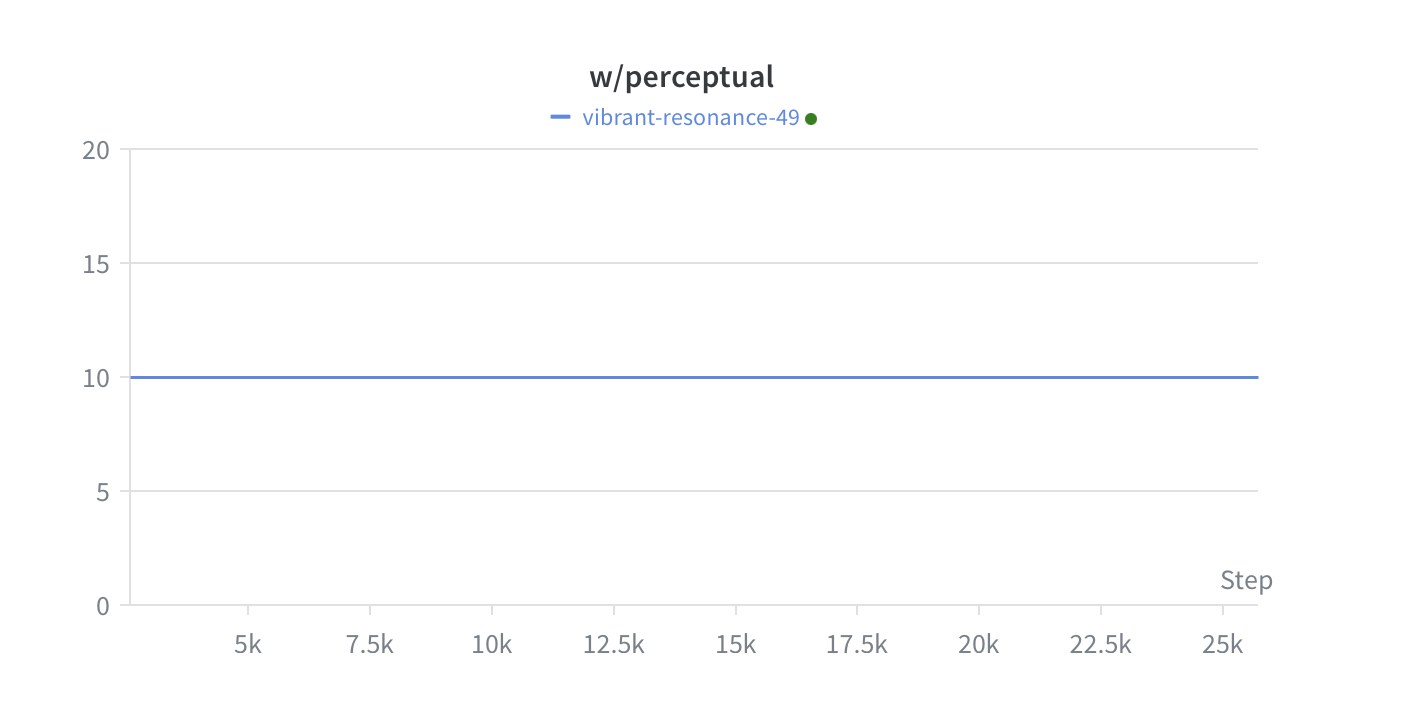
\includegraphics[width=0.95\textwidth]{charts/chart_20.png}
\caption{Metric Chart 20 / Metrik Grafiği 20}
\end{figure}
\clearpage
\begin{figure}[!htb]
\centering
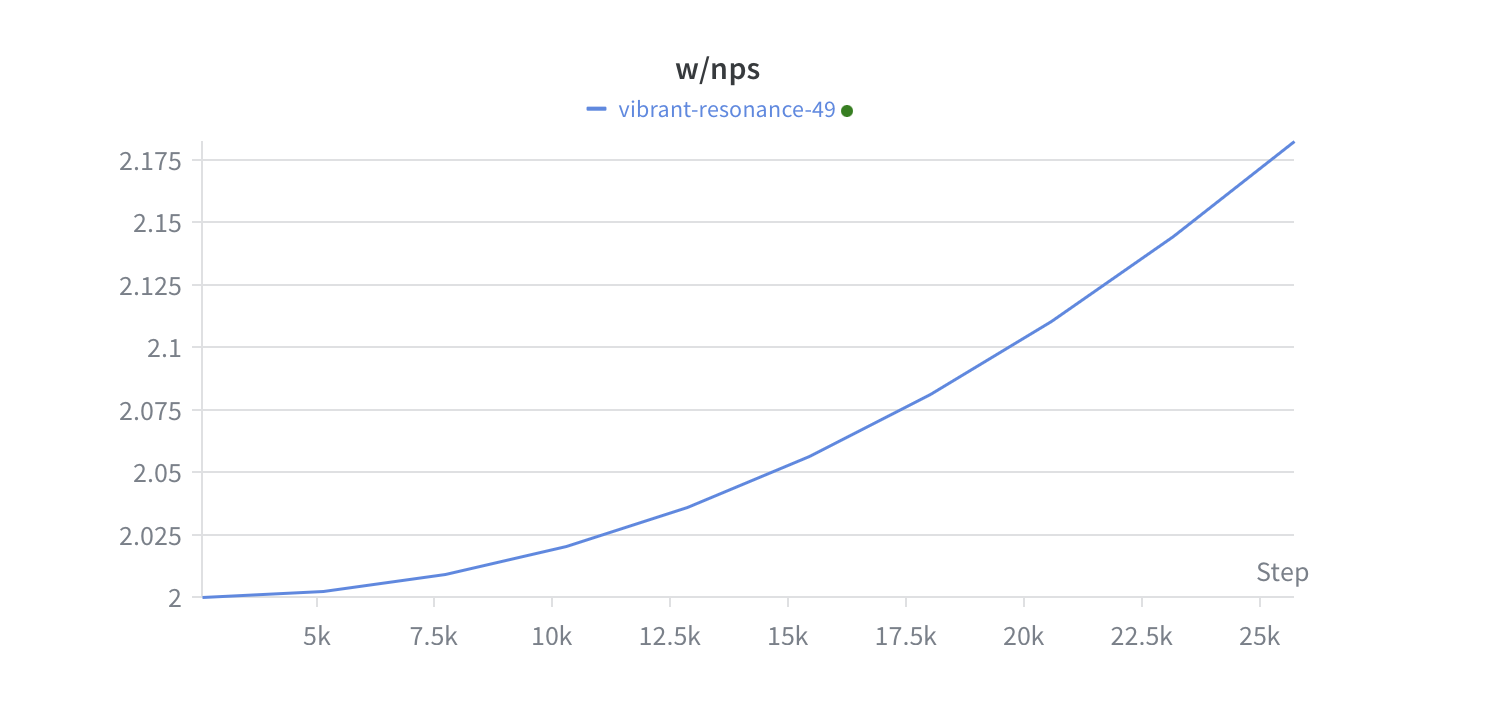
\includegraphics[width=0.95\textwidth]{charts/chart_21.png}
\caption{Metric Chart 21 / Metrik Grafiği 21}
\end{figure}
\begin{figure}[!htb]
\centering
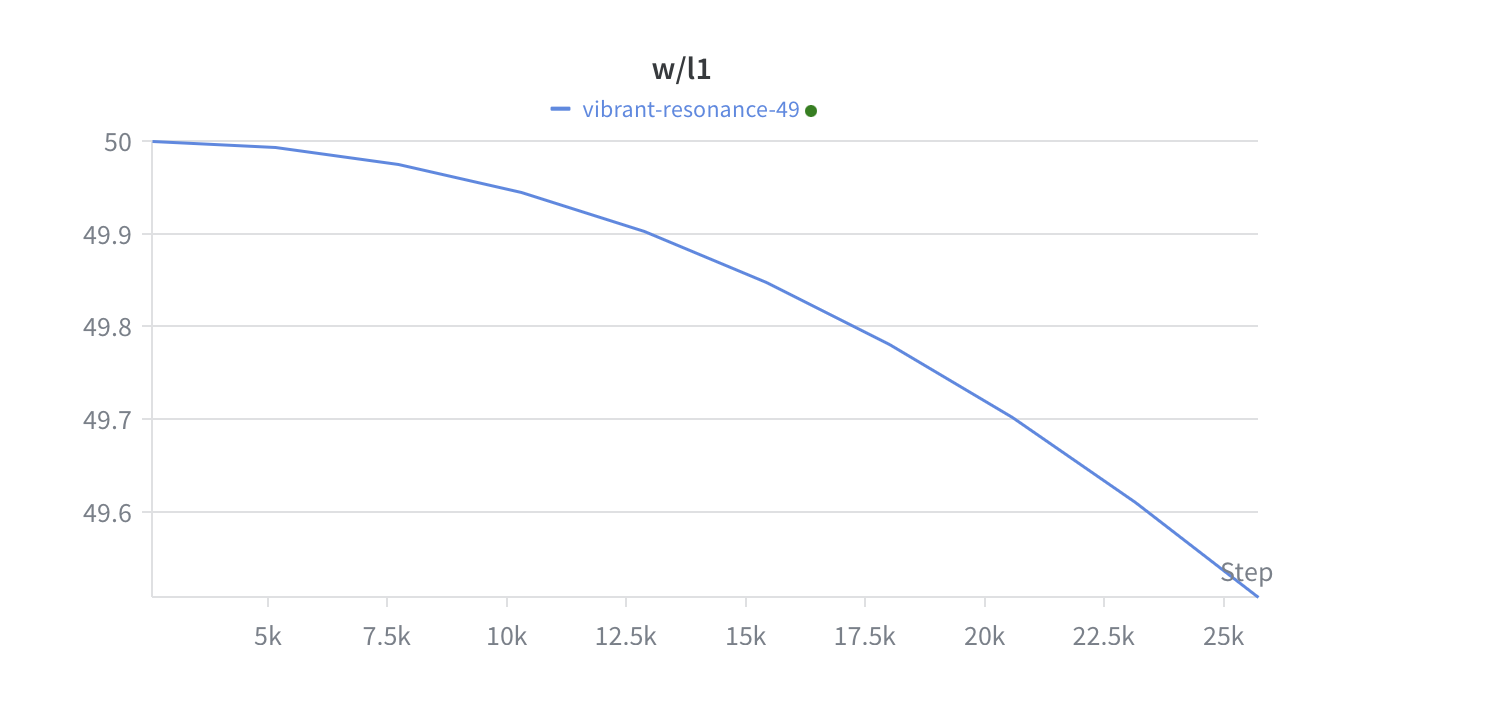
\includegraphics[width=0.95\textwidth]{charts/chart_22.png}
\caption{Metric Chart 22 / Metrik Grafiği 22}
\end{figure}
\clearpage
\begin{figure}[!htb]
\centering
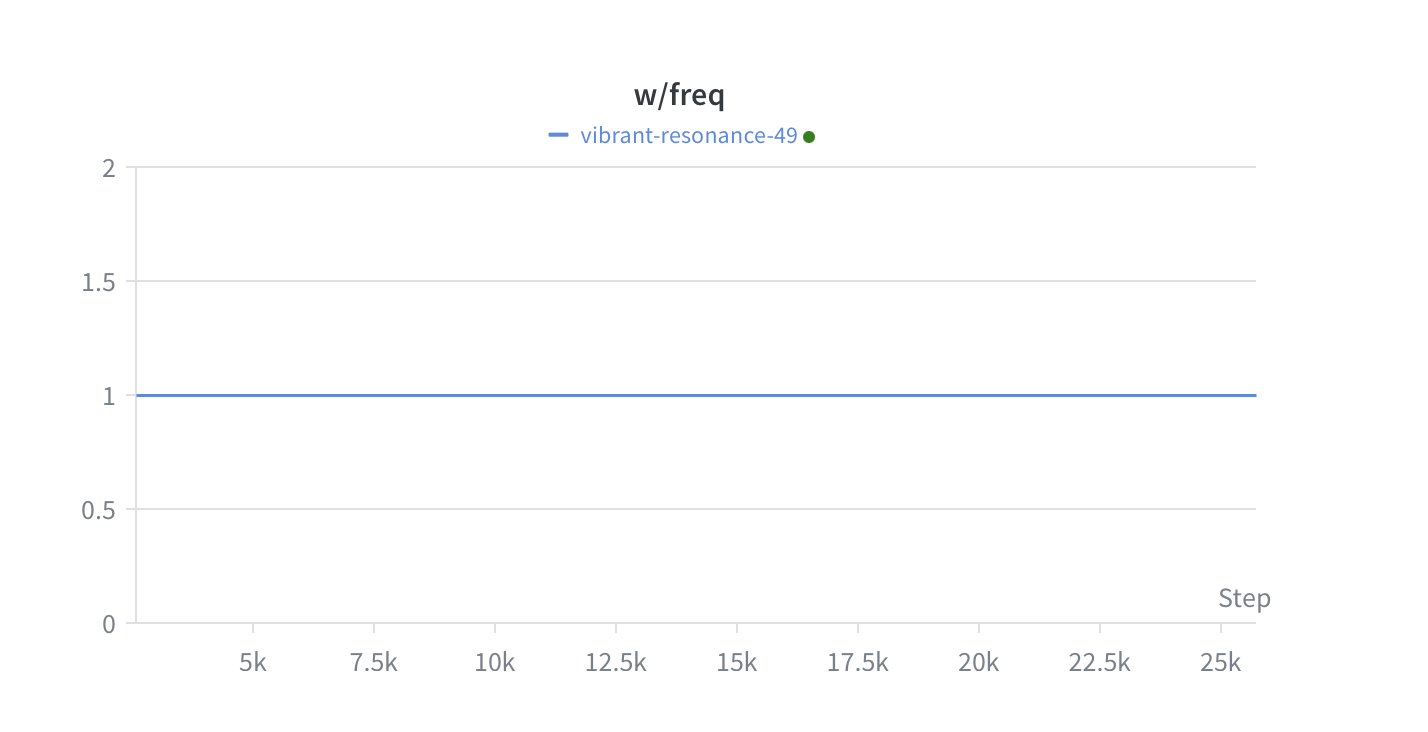
\includegraphics[width=0.95\textwidth]{charts/chart_23.png}
\caption{Metric Chart 23 / Metrik Grafiği 23}
\end{figure}
\begin{figure}[!htb]
\centering
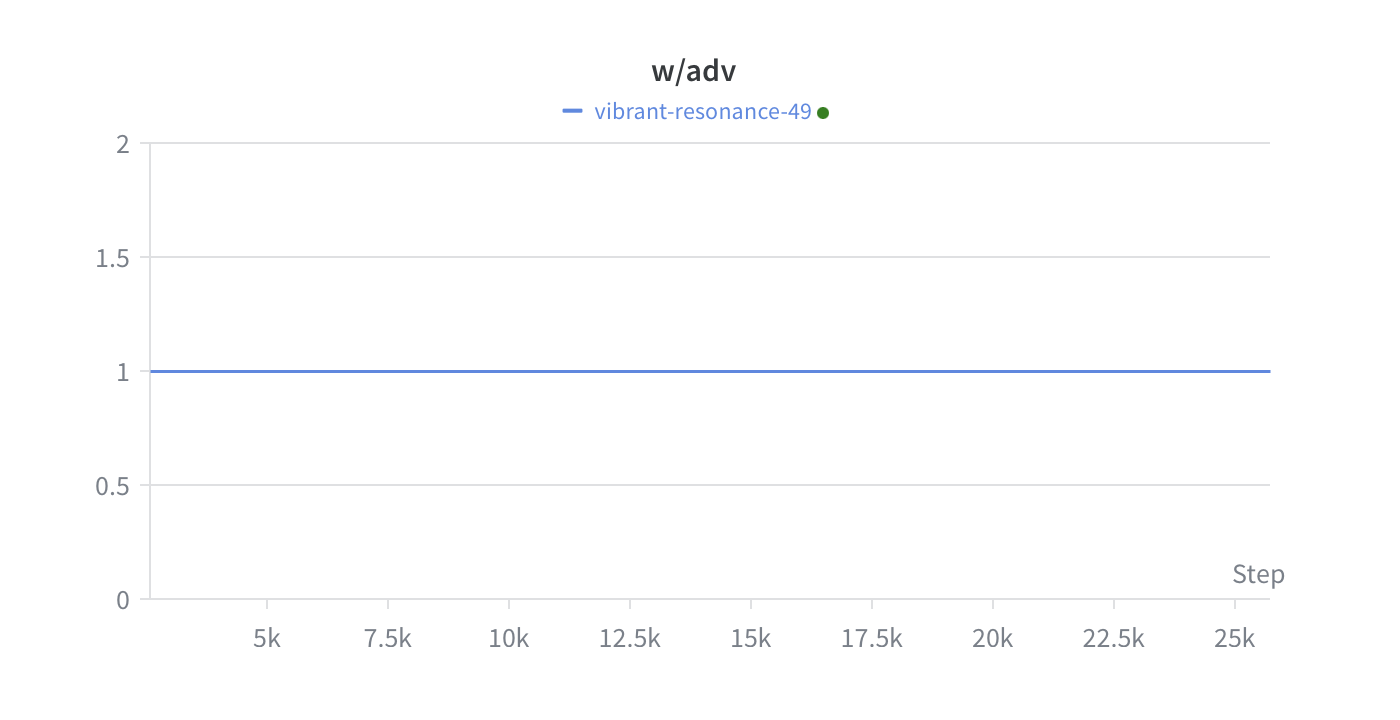
\includegraphics[width=0.95\textwidth]{charts/chart_24.png}
\caption{Metric Chart 24 / Metrik Grafiği 24}
\end{figure}
\clearpage

\clearpage
\section{Qualitative Visual Progression / Niteliksel Görsel Gelişim}
\textbf{EN:} To evaluate visual improvements and detect potential issues like mode collapse or checkerboard artifacts, the progression of generated images across 5 key training steps is presented below.\\
\textbf{TR:} Görsel iyileşmeleri değerlendirmek ve mod çökmesi (mode collapse) veya dama tahtası (checkerboard) artefaktları gibi olası sorunları tespit etmek için, üretilen görüntülerin 5 temel eğitim adımı boyunca gelişimi aşağıda sunulmuştur.

\subsection{Sample 1 Generation Over Time / Örnek 1 Görsel Gelişimi}
\begin{figure}[!htb]
\centering
\minipage{0.48\textwidth}
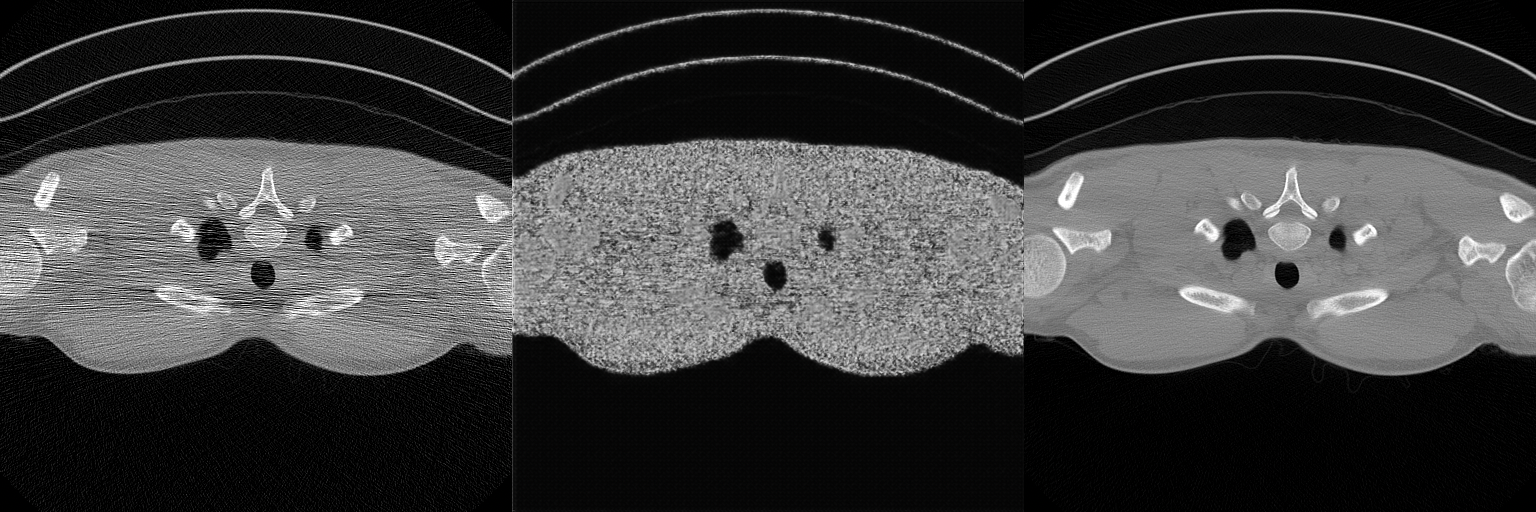
\includegraphics[width=\linewidth]{images/Image_1_Step_0.png}
\caption*{Step 0}
\endminipage\hfill
\minipage{0.48\textwidth}
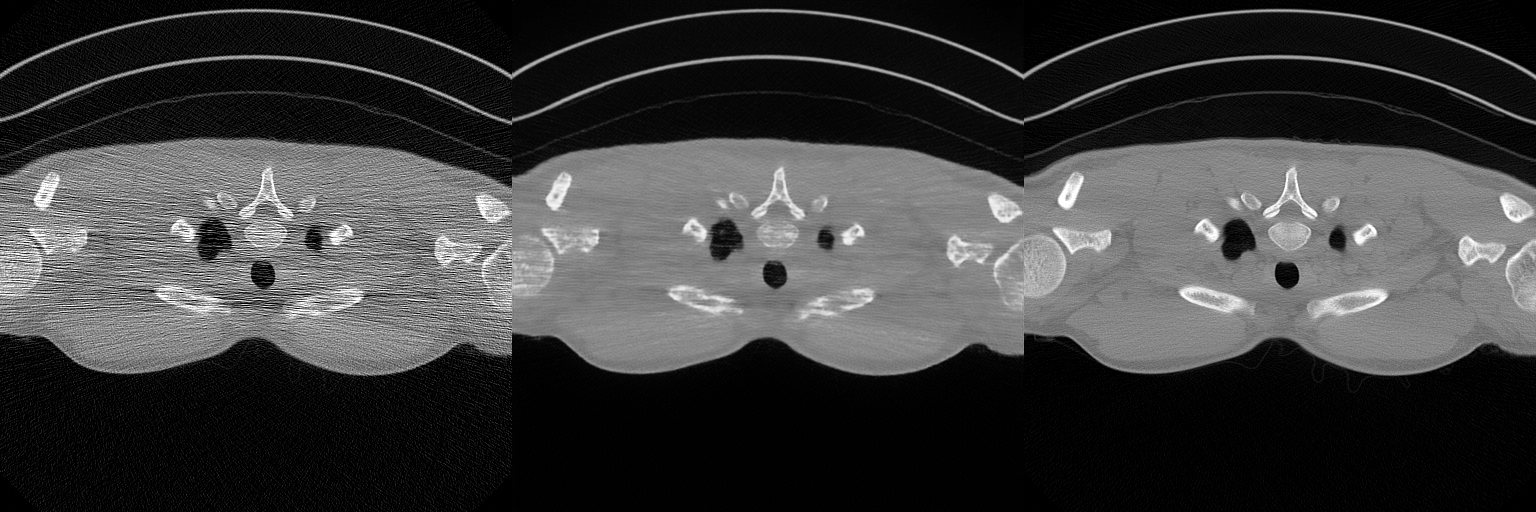
\includegraphics[width=\linewidth]{images/Image_1_Step_5144.png}
\caption*{Step 5144}
\endminipage
\vspace{1em}

\minipage{0.48\textwidth}
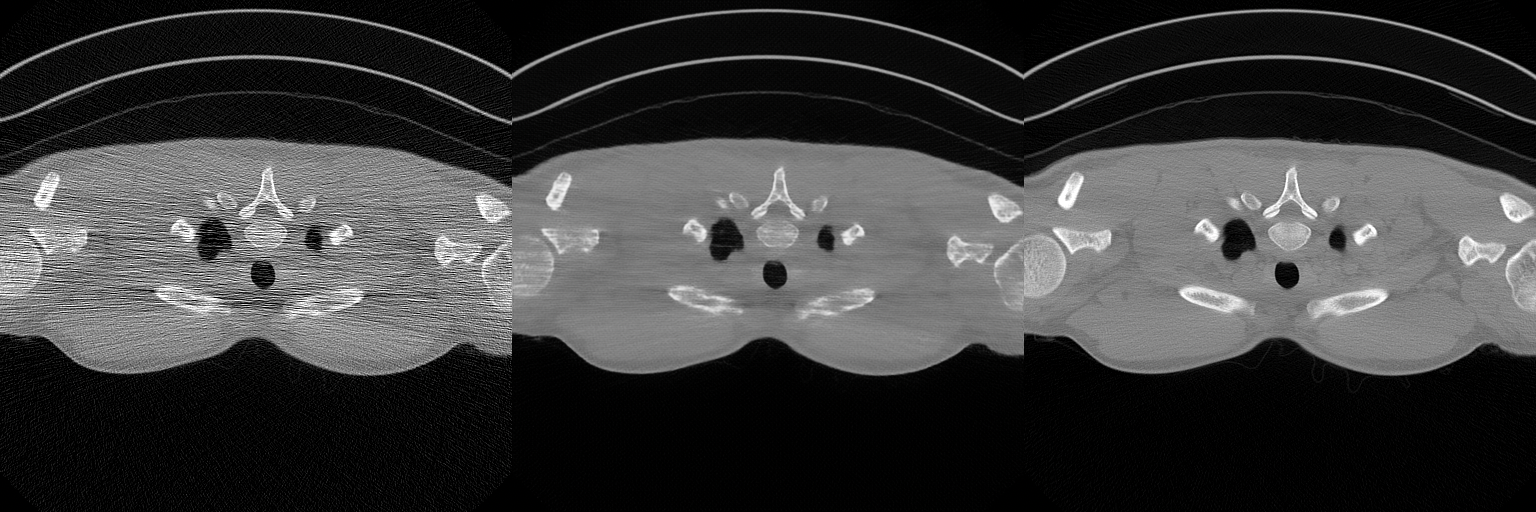
\includegraphics[width=\linewidth]{images/Image_1_Step_10288.png}
\caption*{Step 10288}
\endminipage\hfill
\minipage{0.48\textwidth}
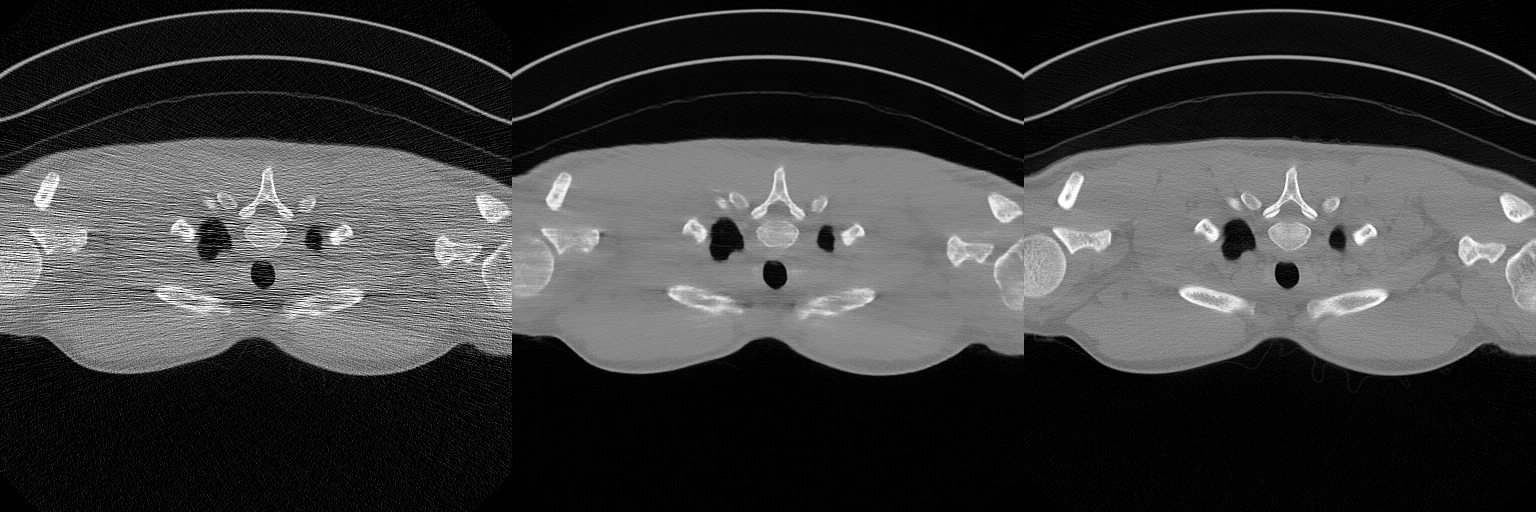
\includegraphics[width=\linewidth]{images/Image_1_Step_15432.png}
\caption*{Step 15432}
\endminipage
\vspace{1em}

\minipage{0.48\textwidth}
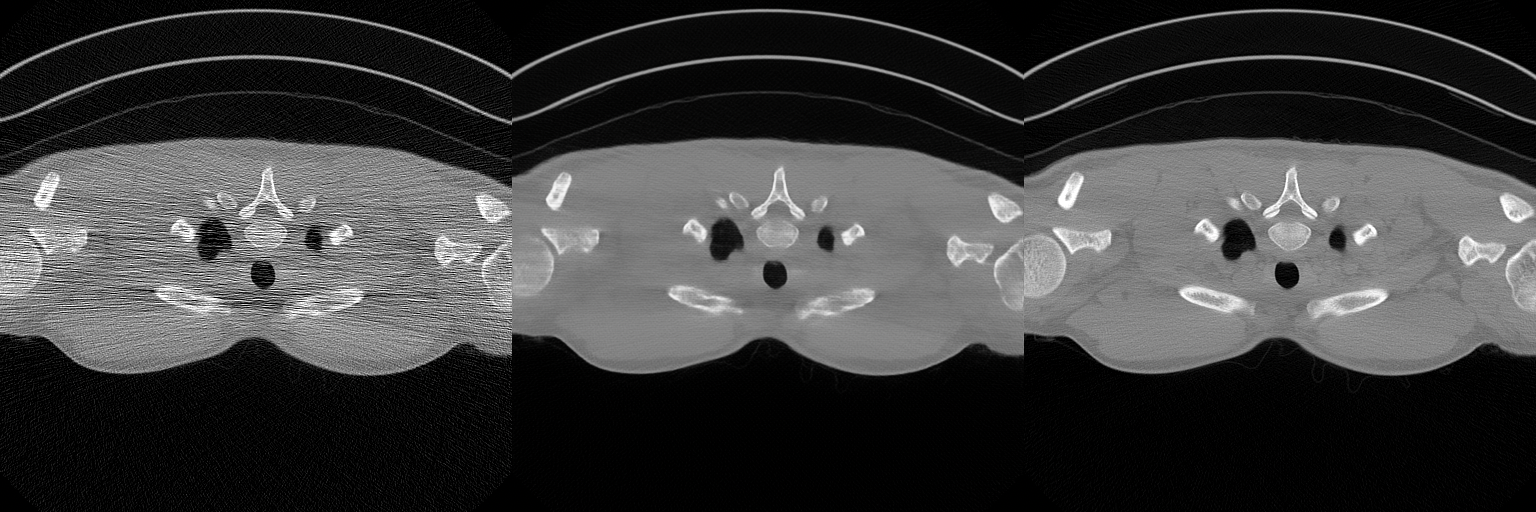
\includegraphics[width=\linewidth]{images/Image_1_Step_20576.png}
\caption*{Step 20576}
\endminipage
\caption{Progression of Image 1 / Örnek 1 Gelişimi}
\end{figure}
\clearpage
\subsection{Sample 2 Generation Over Time / Örnek 2 Görsel Gelişimi}
\begin{figure}[!htb]
\centering
\minipage{0.48\textwidth}
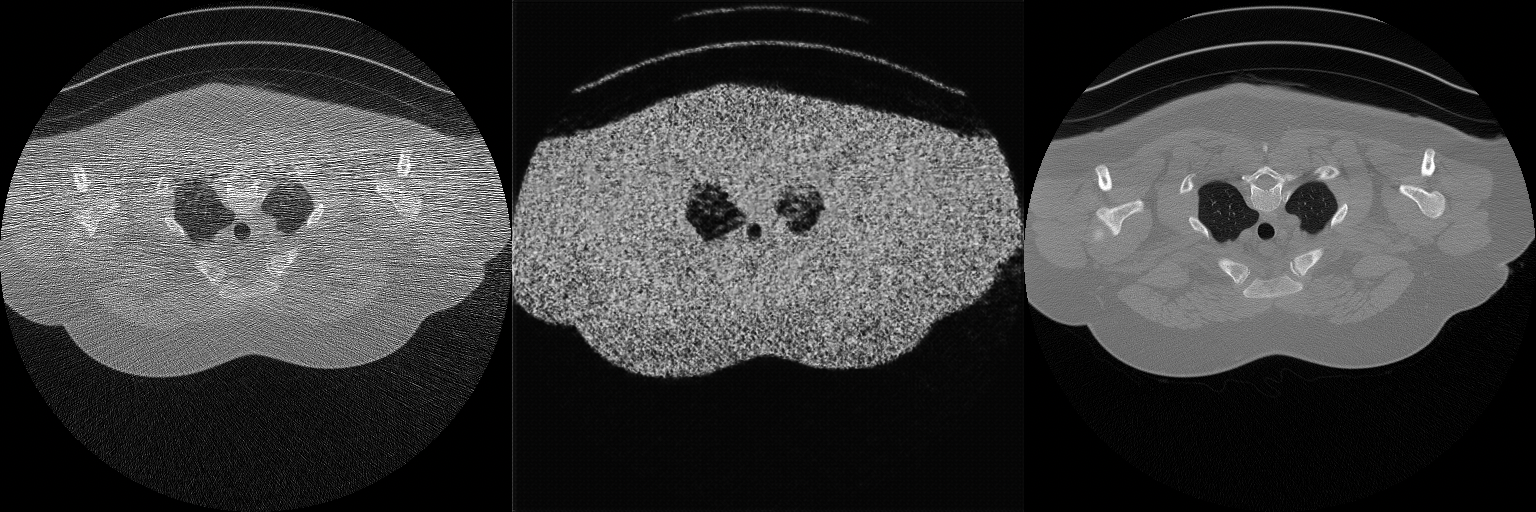
\includegraphics[width=\linewidth]{images/Image_2_Step_0.png}
\caption*{Step 0}
\endminipage\hfill
\minipage{0.48\textwidth}
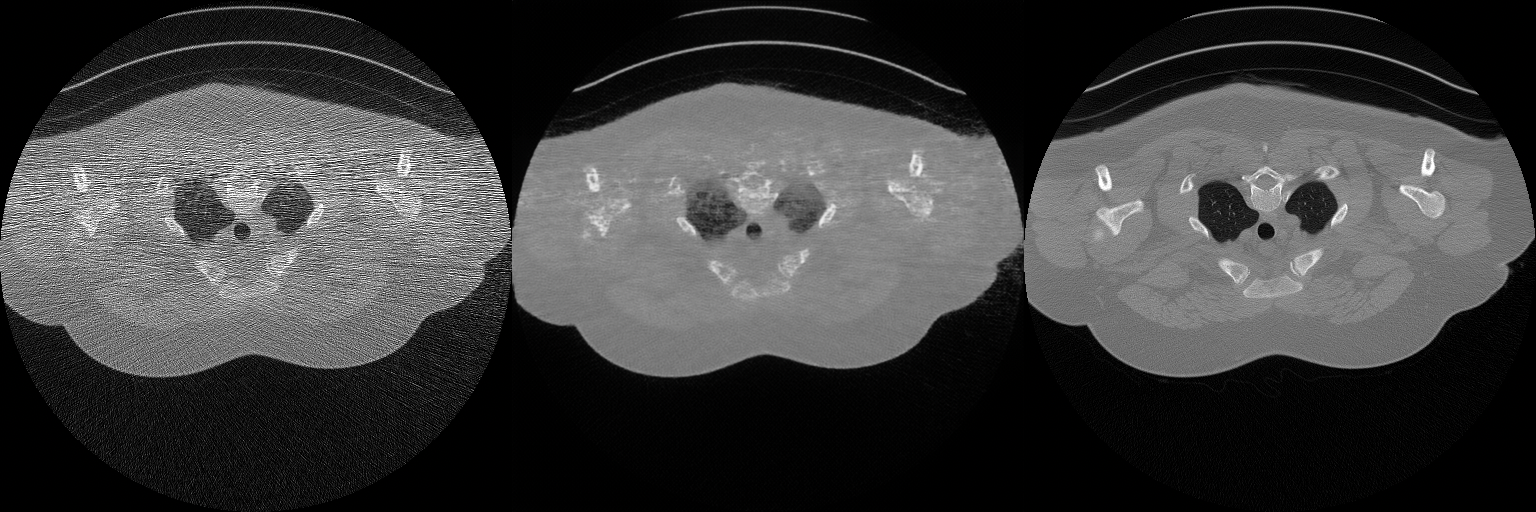
\includegraphics[width=\linewidth]{images/Image_2_Step_5144.png}
\caption*{Step 5144}
\endminipage
\vspace{1em}

\minipage{0.48\textwidth}
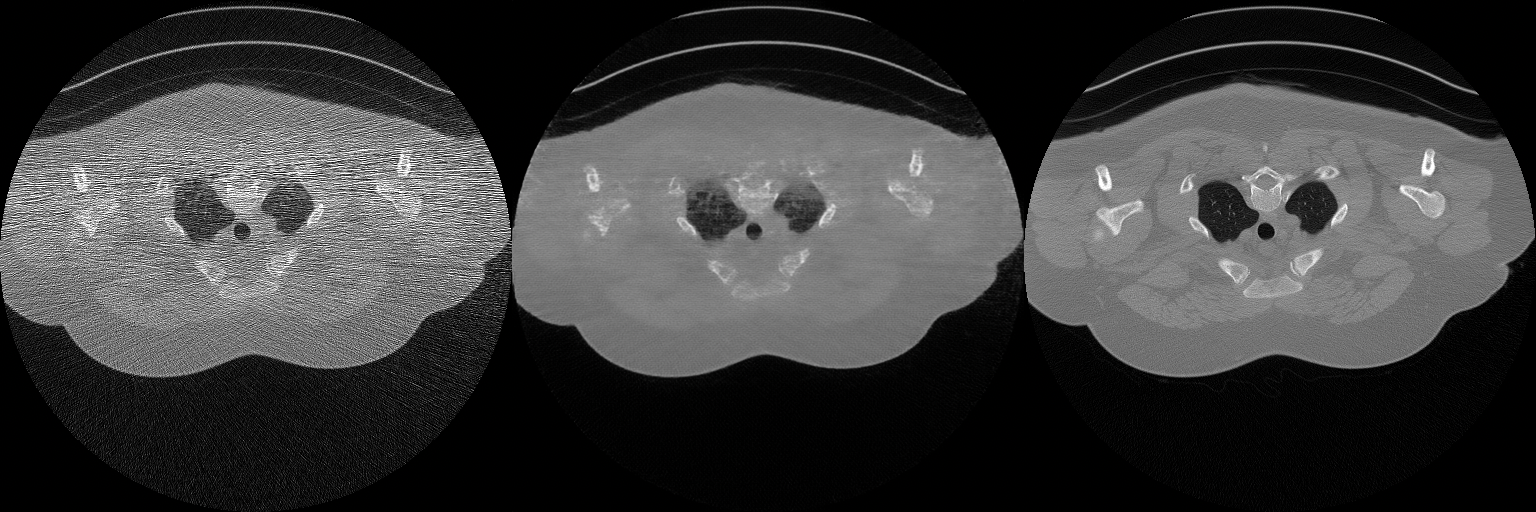
\includegraphics[width=\linewidth]{images/Image_2_Step_10288.png}
\caption*{Step 10288}
\endminipage\hfill
\minipage{0.48\textwidth}
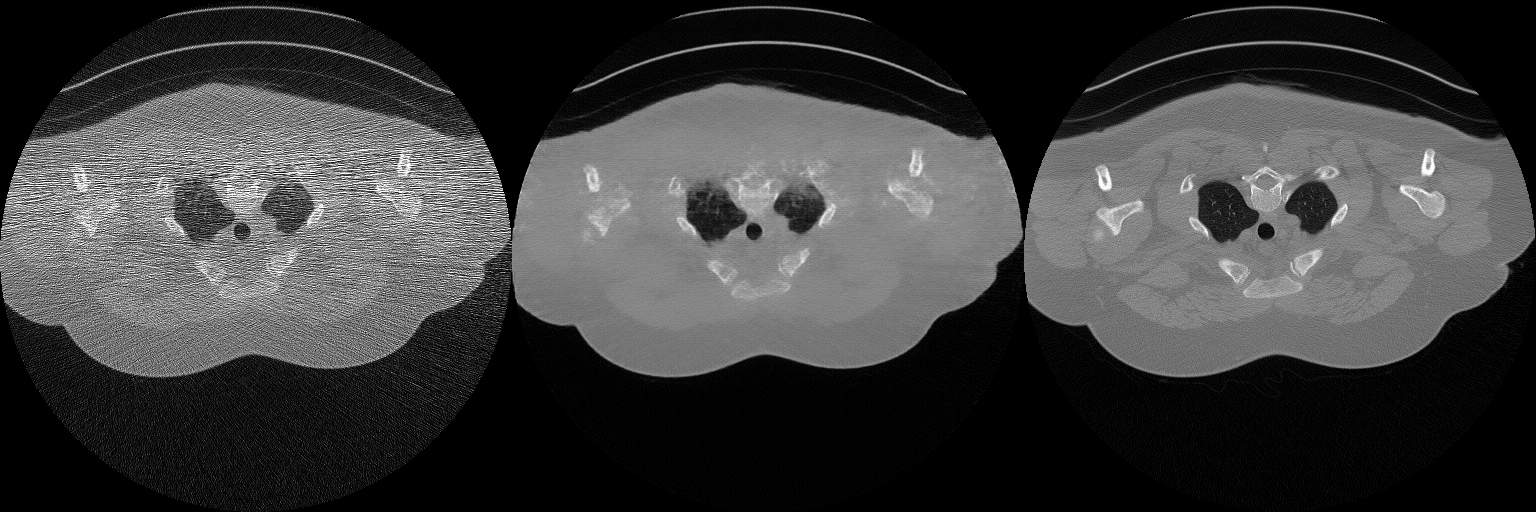
\includegraphics[width=\linewidth]{images/Image_2_Step_15432.png}
\caption*{Step 15432}
\endminipage
\vspace{1em}

\minipage{0.48\textwidth}
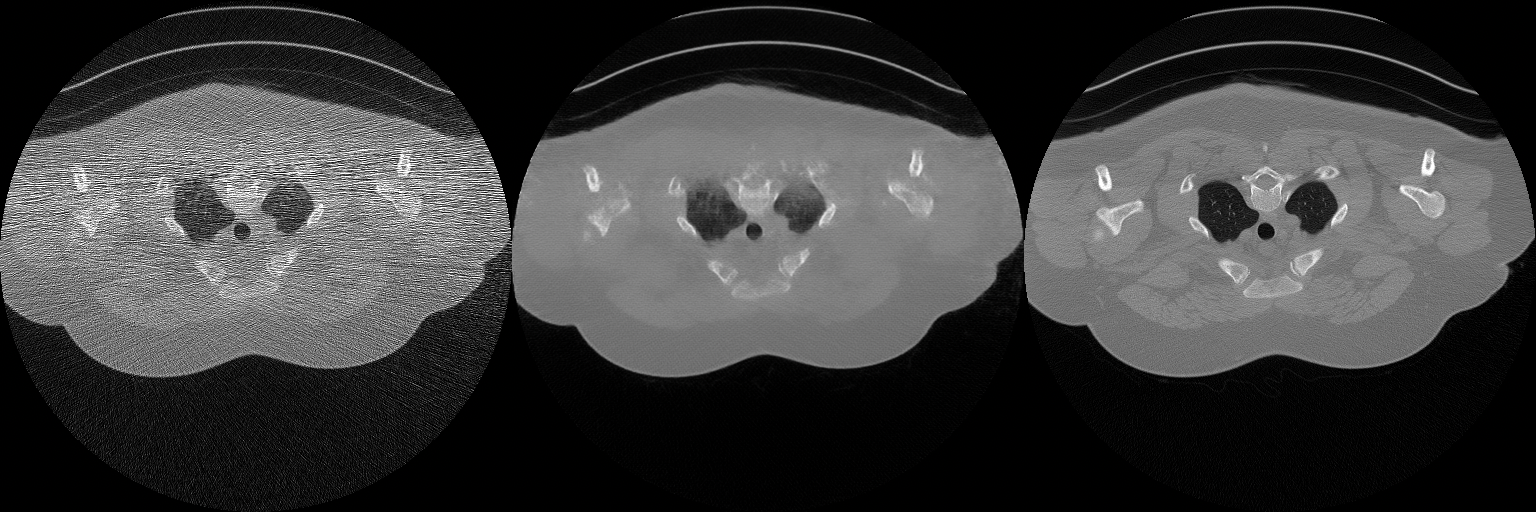
\includegraphics[width=\linewidth]{images/Image_2_Step_20576.png}
\caption*{Step 20576}
\endminipage
\caption{Progression of Image 2 / Örnek 2 Gelişimi}
\end{figure}
\clearpage
\subsection{Sample 3 Generation Over Time / Örnek 3 Görsel Gelişimi}
\begin{figure}[!htb]
\centering
\minipage{0.48\textwidth}
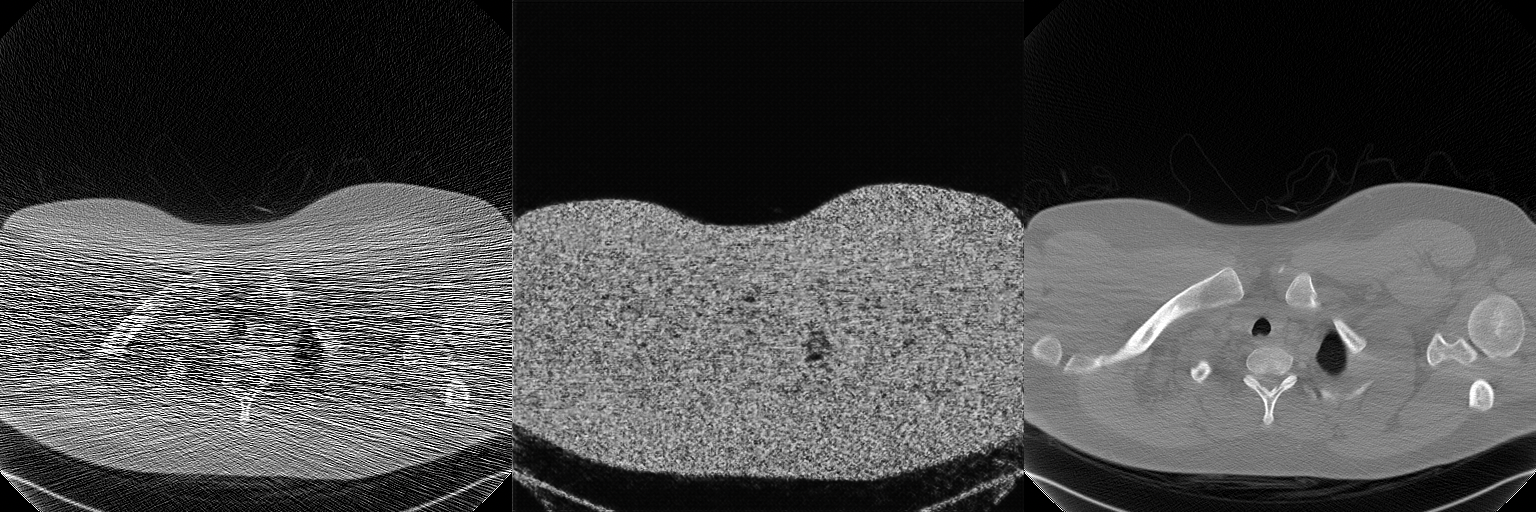
\includegraphics[width=\linewidth]{images/Image_3_Step_0.png}
\caption*{Step 0}
\endminipage\hfill
\minipage{0.48\textwidth}
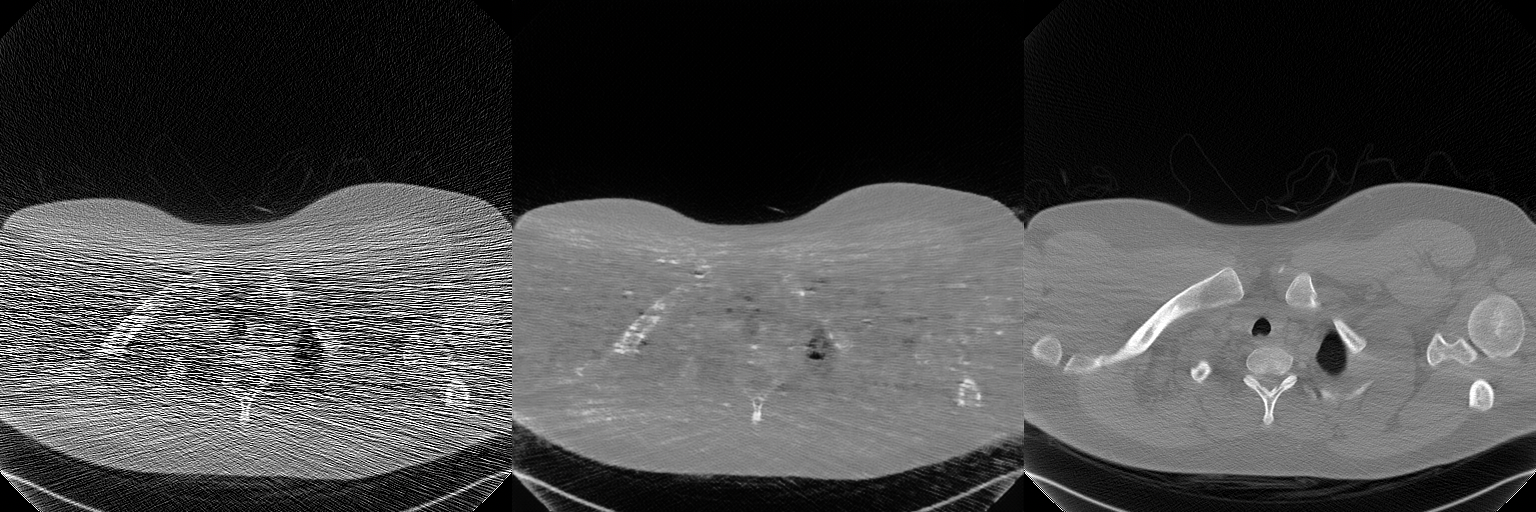
\includegraphics[width=\linewidth]{images/Image_3_Step_5144.png}
\caption*{Step 5144}
\endminipage
\vspace{1em}

\minipage{0.48\textwidth}
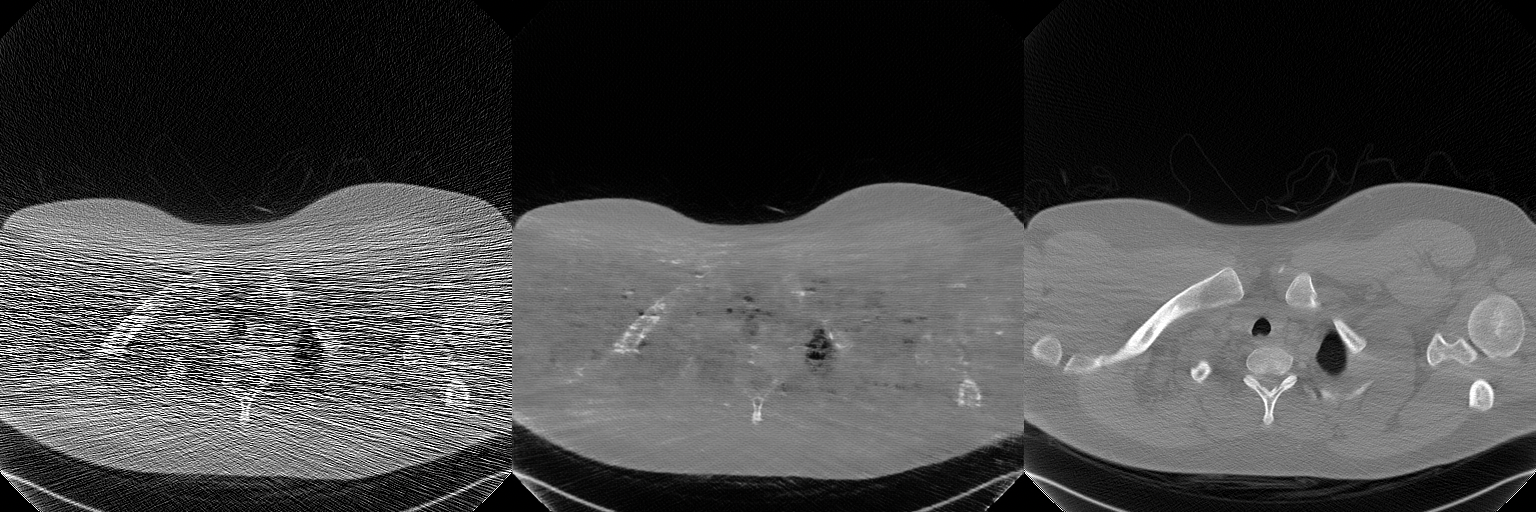
\includegraphics[width=\linewidth]{images/Image_3_Step_10288.png}
\caption*{Step 10288}
\endminipage\hfill
\minipage{0.48\textwidth}
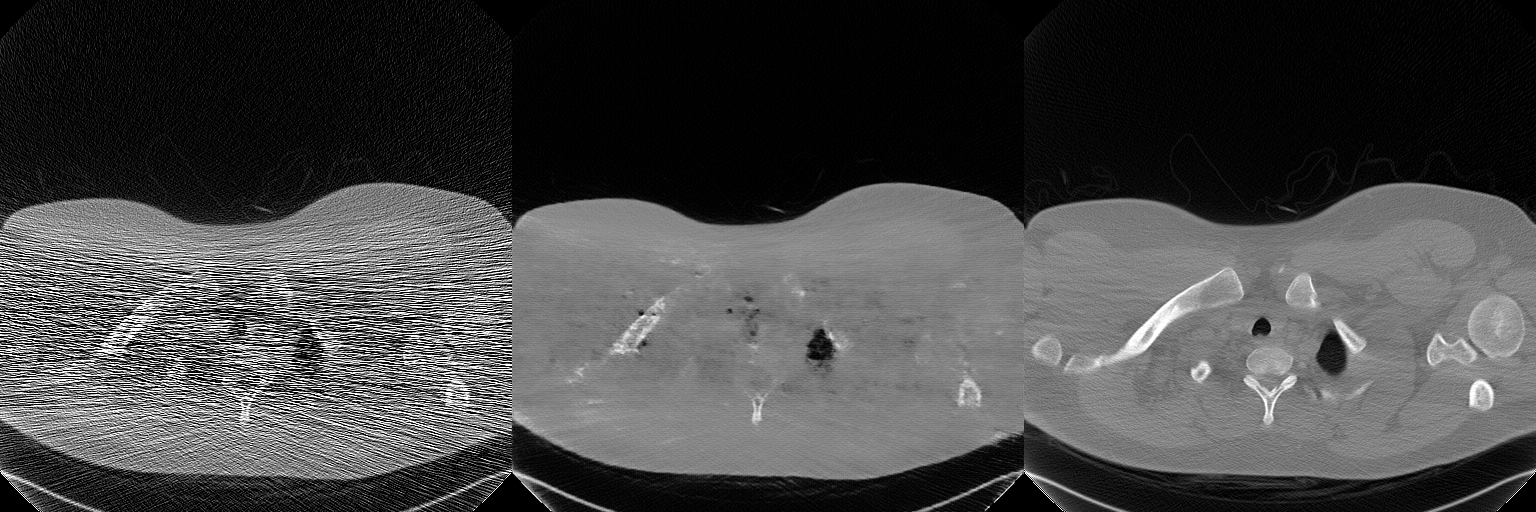
\includegraphics[width=\linewidth]{images/Image_3_Step_15432.png}
\caption*{Step 15432}
\endminipage
\vspace{1em}

\minipage{0.48\textwidth}
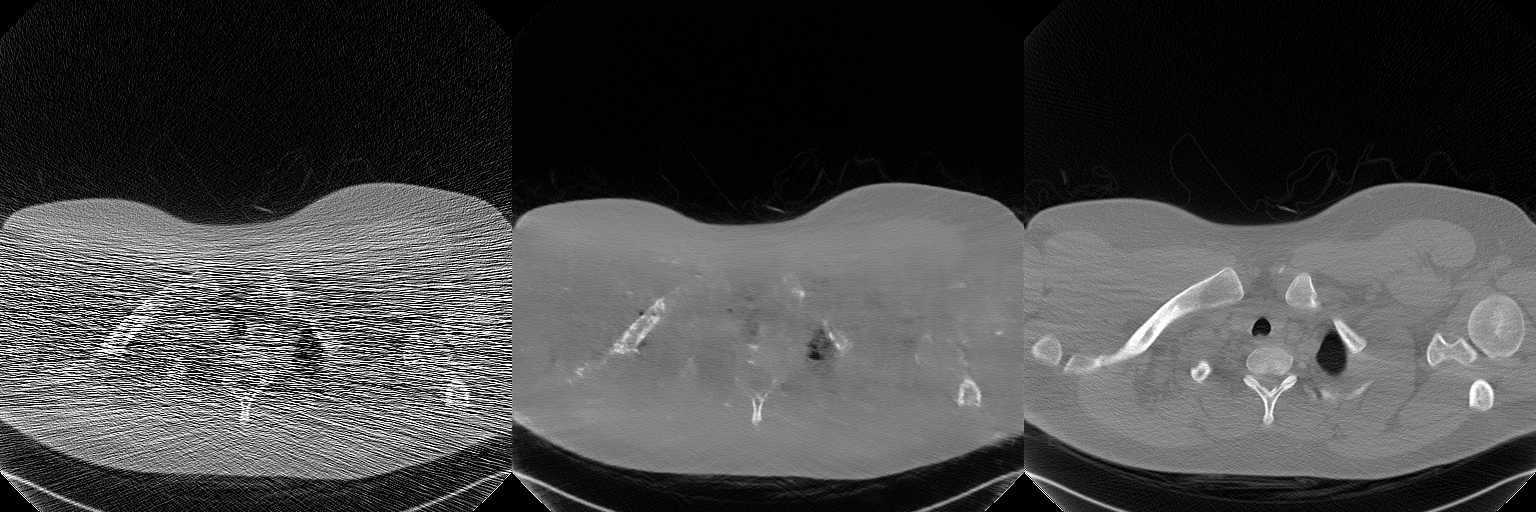
\includegraphics[width=\linewidth]{images/Image_3_Step_20576.png}
\caption*{Step 20576}
\endminipage
\caption{Progression of Image 3 / Örnek 3 Gelişimi}
\end{figure}
\clearpage

\vspace{2em}

\noindent\fbox{\parbox{\dimexpr\textwidth-2\fboxsep-2\fboxrule\relax}{
\textbf{Agent Analysis Prompt: Final Verdict Required / Analiz Ajanı İstemi: Nihai Karar Gerekli} \\
\textbf{EN Instructions:}
\begin{itemize}
    \item \textbf{Loss Stability:} Are the generator and discriminator losses oscillating, diverging, or stabilizing? Review the Quantitative Metrics sections.
    \item \textbf{Visual Quality Assessment:} Do the images show significant detail improvement across the 5 steps? Are there persistent checkerboard artifacts or signs of mode collapse?
    \item \textbf{Actionable Recommendation:} Based on your analysis, should the training continue as-is, be stopped, or require architectural/hyperparameter adjustments?
\end{itemize}
\textbf{TR Talimatlar:}
\begin{itemize}
    \item \textbf{Kayıp İstikrarı:} Üretici (generator) ve ayırt edici (discriminator) kayıpları dalgalanıyor mu, uzaklaşıyor mu (diverge) yoksa dengeleniyor mu?
    \item \textbf{Görsel Kalite Değerlendirmesi:} Görüntüler 5 adım boyunca önemli detay iyileştirmeleri gösteriyor mu? Kalıcı dama tahtası (checkerboard) bozulmaları veya mod çökmesi (mode collapse) belirtileri var mı?
    \item \textbf{Uygulanabilir Öneri:} Analizinize dayanarak, eğitim olduğu gibi devam mı etmeli, durdurulmalı mı yoksa mimari/hiperparametre ayarları mı gerektiriyor?
\end{itemize}
\textbf{Provide your comprehensive final verdict and justification to the human researcher. / Kapsamlı nihai kararınızı ve gerekçenizi araştırmacıya sunun.}
}}

\nocite{*}
\bibliographystyle{unsrt}
\bibliography{bibliography}
\end{document}
